\documentclass{article}

% Packages
\usepackage[margin=1.5cm, includefoot, footskip=30pt]{geometry}
\usepackage{hyperref}
\usepackage{multicol}
\usepackage{booktabs}
\usepackage{xstring}
\usepackage{subcaption}
\usepackage{graphicx}
\usepackage{amsmath}
\usepackage{standalone}
\usepackage{fancyvrb}

\usepackage{pdflscape}

\usepackage{tikz}
\usetikzlibrary{calc, shapes, patterns}

\usepackage[backend=biber, firstinits=false, backref=false, url=true,
            isbn=true, style=numeric]{biblatex}
\addbibresource{bibliography.bib}

% Title
\title{Reinforcement Learning Produces Dominant Strategies for the
Iterated Prisoner's Dilemma}
\author{Marc Harper \and Vincent Knight} % TODO Authors
\date{}


\begin{document}

\maketitle

\begin{abstract}
    We present tournament results and several powerful strategies for the Iterated
    Prisoner's Dilemma created using reinforcement learning techniques
    (evolutionary and particle swarm algorithms). These strategies are
    trained to perform well against a corpus of over 100 distinct
    opponents, including many well-known strategies from the literature, and all
    the trained strategies win standard tournaments against the total collection
    of other opponents. We also trained variants to win noisy tournaments.
\end{abstract}

\section{Introduction}\label{sec:introduction}

The Axelrod library \cite{knight2016open} is an open source software for
conducting iterated prisoner's dilemma (IPD) research with reproducibilty as a
principal goal. Written in the Python programming language, to date over the
library contains source code contibuted by over 50 individuals from a variety
of geographic locations and technical backgrounds. The library is supported by
a comprehensive test suite that covers all the intended behaviors of the
strategies in the library, as well as the features that conduct matches,
tournaments, and population dynamics.

As of version 3.0.0, the library contains over 200 strategies,
many from the scientific literature, including classic strategies like Win Stay
Lose Shift \cite{nowak1993strategy} and previous tournament winners such as
OmegaTFT \cite{slany2007some}, Adaptive Pavlov \cite{li2007design}, and
ZDGTFT2 \cite{stewart2012extortion}.

% TODO: discuss earlier tournaments

In this work we utilize the collection of strategies in the Axelrod library
to train new strategies specifically to win IPD tournaments. We train these
strategies using generic strategy archetypes based on e.g. finite state
machines, arriving at particularly effective parameter choices through
evolutionary or particle swarm algorithms. There are several
previous publications that use evolutionary algorithms to
evolve IPD strategies in various circumstances
\cite{ashlock2006training, ashlock2015multiple, ashlock2006changes,
      ashlock2014shaped, ashlock2014evolution, barlow2015varying,
      fogel1993evolving, marks1989niche, sudo2015effects,
      vassiliades2010multiagent}. See also \cite{gaudesi2016exploiting} for a
strategy trained to win against a collection of well-known IPD opponents and see
\cite{franken2005particle} for a prior use of particle swarm algorithms. Our
results are unique in that we are able to train against a large collection of
well-known strategies available in the scientific literature. Crucially, the
software used in this work is openly available and can be used to train strategies
in the future in a reliable manner, with confidence that the opponent strategies
are correctly implemented and documented. Moreover, as of the time of writing,
we claim that this work contains the best known strategies for the iterated
prisoner's dilemma.

\section{The Strategy Archetypes}

The Axelrod library now contains many parametrised strategies trained using
machine learning
methods. Most are deterministic, use many rounds of memory, and perform
extremely well in tournaments.

The various archetypes will be described in the following sections.

\subsection{LookerUp}

The first strategy trained with reinforcement learning in the library is based
on lookup tables. The strategy encodes a set of deterministic responses
based on the opponent's first $n_1$ moves, the opponent's last $m_1$ moves, and
the players last $m_2$ moves. If $n_1 > 0$ then the player has infinite memory
depth, otherwise it has depth $\max{m_1, m_2}$. Although we tried various
combinations of $n_1, m_1,$ and $m_2$, the best performance at the time of
training was obtained for $n_1 = m_1 = m_2 = 2$ and generally for $n_1 > 0$.
The library includes a strategy
called EvolvedLookerUp2\_2\_2 which is among the top strategies in the library.

This archetype can be used to train deterministic memory-$n$ strategies with the
parameters $n_1=0$ and $m_1=m_2=n$. For $n=1$, the resulting strategy cooperates
if the last round was mutual cooperation and defects otherwise.

Two strategies in the library, Winner12 and Winner21, from \cite{Mathieu2015},
are based on lookup tables for $n_1 = 0$, $m_1 = 1$, and $m_2=2$. The strategy
Winner12 emerged in less than 10 generations of training in our framework using
a score maximizing objective. Strategies nearly identical to Winner21 arise
from training with a Moran process objective.

\subsection{PSO Gambler}

PSO Gambler is a stochastic variant of LookerUp. Instead of deterministically
encoded moves the lookup table emits probabilities which are
used to choose cooperation or defection. The library includes a player trained
with $n_1 = m_1 = m_2 = 2$ that is \emph{mostly deterministic}, with most of the
probabilities being 0 or 1. At one time this strategy outperformed
EvolvedLookerUp2\_2\_2.

This strategy type can be used to train arbitrary memory-$n$ strategies. A
memory one strategy called PSO Gambler Mem 1 was trained, with
probabilities $(\text{Pr}(\text{C}\;|\;\text{CC}),
                \text{Pr}(\text{C}\;|\;\text{CD}),
                \text{Pr}(\text{C}\;|\;\text{DC}),
                \text{Pr}(\text{C}\;|\;\text{DD})) = (1, 0.5217, 0, 0.121)$.
Though it performs well in standard tournaments (see
Table~\ref{tbl:standard_score})
it is not as good as the longer memory strategies, and is bested by a similar
strategy that also uses the first round of play: PSO Gambler 1 1 1.

These strategies are trained with a particle swarm algorithm rather than an
evolutionary algorithm (though the former would suffice). Particle swarm
algorithms have been used to trained IPD strategies previously
\cite{franken2005particle}.

\subsection{ANN: Single Layer Artificial Neural Network}

Strategies based on artificial neural networks can also be trained with an
evolutionary algorithm. A variety of features are computed from the history
of play such as the opponents trailing moves, the total number of cooperations
of the player and the opponent, and several others, which are then input
into a feed forward neural network with one layer and user-supplied width.
An inner layer with just five nodes performs quite well in both deterministic and
noisy tournaments. The output of the ANN used in this work is deterministic;
a stochastic variant that outputs probabilities rather than exact moves could
be easily created.

\subsection{Finite State Machines}

We used strategies based on finite state machines to create a number of
strategies. These strategies are deterministic and are efficient computationally.
In each round of play the strategy selects an action based on the current state
and the opponent's last action, transitioning to a new state for the next round.
These strategies can encode a variety
of other strategies, including classic strategies like TitForTat, 
handshake strategies, and grudging strategies that always defect after
an opponent defection.

% TODO: One or more FSM diagrams

\subsection{Hidden Markov Models}

We also trained stochastic versions of finite state machine players called
hidden Markov model players or HMMs. Like the finite state machines, these
strategies also encode an internal
state with probabilistic transitions based on the prior round of play to other
states and cooperate or defect with various probabilities at each state. These
are the best performing stochastic strategies in the library but take longer
to train due to their stochasticity.

\subsection{Meta Strategies}

Last but not least there are several strategies based on ensemble methods that
are common in machine learning called Meta strategies. These strategies are
composed of a team of other strategies. In each round, each member of the team
is polled for its desired next
move. The ensemble then selects the next move based on a rule, such as the
consensus vote in the case of MetaMajority or the best individual performance
in the case of MetaWinner. These strategies were among the best in the library
before the inclusion of those trained by reinforcement learning.

Because these strategies inherit many of the properties of the strategies
on which they are based, including using the match length to defect on the last
rounds of play, these strategies were omitted from the tournament results.

\section{Results}

\subsection{Standard Tournament}

We conducted a tournament with a large collection of strategies from the Axelrod
library, including some additional parametrized strategies (e.g. various parameter
choices for Generous Tit For Tat). These are listed in
Appendix~\ref{app:list_of_players}.
The top 11 performing strategies by median payoff are all strategies trained to maximize
% TODO Potentially modify this as more repetitions are analysed.
total payoff against a subset of the strategies (Table~\ref{tbl:standard_score}).
The next strategy is Desired Belief Strategy (DBS)
% TODO Add reference for DBS
which actively analyzes the opponent and responds
accordingly. The next two strategies are Winner12, based on a lookup table,
Fool Me Once, a grudging strategy that defects indefinitely on
the second defection, and Omega Tit For Tat \cite{Slany2007}.
All strategies in the tournament follow a simple set of
rules in accordance with earlier tournaments:

\begin{itemize}
  \item Players are unaware of the number of turns in a match
  \item Players carry no acquired state between matches
  \item Players cannot observe the outcome of other matches
  \item Players cannot identify their opponent by any label or identifier
  \item Players cannot manipulate or inspect their opponents in any way
\end{itemize}

Any strategy that does not follow these rules, such as a strategy that defects
on the last round of play, was omitted from the tournament presented here (but
not from the training pool).

% Table of best strategies
\begin{table}[!hbtp]
        \centering
        \begin{tabular}{lrrrrrrrrr}
\toprule
{} &   mean &    std &    min &     5\% &    25\% &    50\% &    75\% &    95\% &    max \\
\midrule
EvolvedLookerUp2\_2\_2    &  2.955 &  0.010 &  2.915 &  2.937 &  2.948 &  2.956 &  2.963 &  2.971 &  2.984 \\
Evolved HMM 5           &  2.954 &  0.014 &  2.903 &  2.931 &  2.945 &  2.954 &  2.964 &  2.977 &  3.003 \\
Evolved FSM 16          &  2.952 &  0.013 &  2.900 &  2.930 &  2.944 &  2.953 &  2.962 &  2.973 &  2.993 \\
PSO Gambler 2\_2\_2       &  2.938 &  0.013 &  2.886 &  2.913 &  2.930 &  2.940 &  2.948 &  2.957 &  2.971 \\
Evolved FSM 16 Noise 05 &  2.919 &  0.013 &  2.874 &  2.898 &  2.910 &  2.919 &  2.928 &  2.940 &  2.961 \\
PSO Gambler 1\_1\_1       &  2.912 &  0.023 &  2.810 &  2.873 &  2.896 &  2.912 &  2.927 &  2.950 &  3.012 \\
Evolved ANN 5           &  2.912 &  0.010 &  2.873 &  2.894 &  2.905 &  2.912 &  2.919 &  2.928 &  2.944 \\
Evolved FSM 4           &  2.910 &  0.012 &  2.868 &  2.889 &  2.901 &  2.910 &  2.919 &  2.929 &  2.942 \\
Evolved ANN             &  2.907 &  0.010 &  2.865 &  2.891 &  2.901 &  2.908 &  2.914 &  2.923 &  2.942 \\
PSO Gambler Mem1        &  2.901 &  0.025 &  2.794 &  2.859 &  2.884 &  2.902 &  2.919 &  2.942 &  2.984 \\
Evolved ANN 5 Noise 05  &  2.864 &  0.008 &  2.837 &  2.850 &  2.858 &  2.865 &  2.870 &  2.877 &  2.891 \\
DBS: 0.75, 3, 4, 3, 5   &  2.857 &  0.009 &  2.827 &  2.842 &  2.851 &  2.857 &  2.863 &  2.872 &  2.888 \\
Winner12                &  2.849 &  0.008 &  2.821 &  2.836 &  2.843 &  2.850 &  2.855 &  2.862 &  2.873 \\
Fool Me Once            &  2.844 &  0.008 &  2.820 &  2.831 &  2.838 &  2.844 &  2.850 &  2.857 &  2.882 \\
Omega TFT: 3, 8         &  2.841 &  0.011 &  2.805 &  2.822 &  2.833 &  2.841 &  2.849 &  2.859 &  2.878 \\
\bottomrule
\end{tabular}

        \caption{Standard Tournament: Mean score per turn of top 15 strategies
            (ranked by median over
        \protect50000tournaments).
        The leaderboard is dominated by the machine learning strategies. ~$^{*}$
        indicates that the strategy was trained.}
        \label{tbl:standard_score}
\end{table}

Violin plots showing the distribution of the scores of each strategy (again
ranked by median score) are shown in Figure~\ref{fig:standard_boxplot}.

\begin{landscape}
    \begin{figure}[!hbtp]
        \centering
        \includegraphics[width=\paperwidth]{./assets/standard_scores_boxplots.pdf}
        \caption{Standard Tournament: Mean score per turn (ranked by median
        over
        \protect50000tournaments)}
        \label{fig:standard_boxplot}
    \end{figure}
\end{landscape}

Pairwise payoff results are given as a heatmap (Figure~\ref{fig:standard_heatmap})
which shows that many strategies achieve mutual cooperation. The top performing
strategies never defect first yet are able to exploit weaker strategies that
attempt to defect.

\begin{figure}[!hbtp]
    \centering
    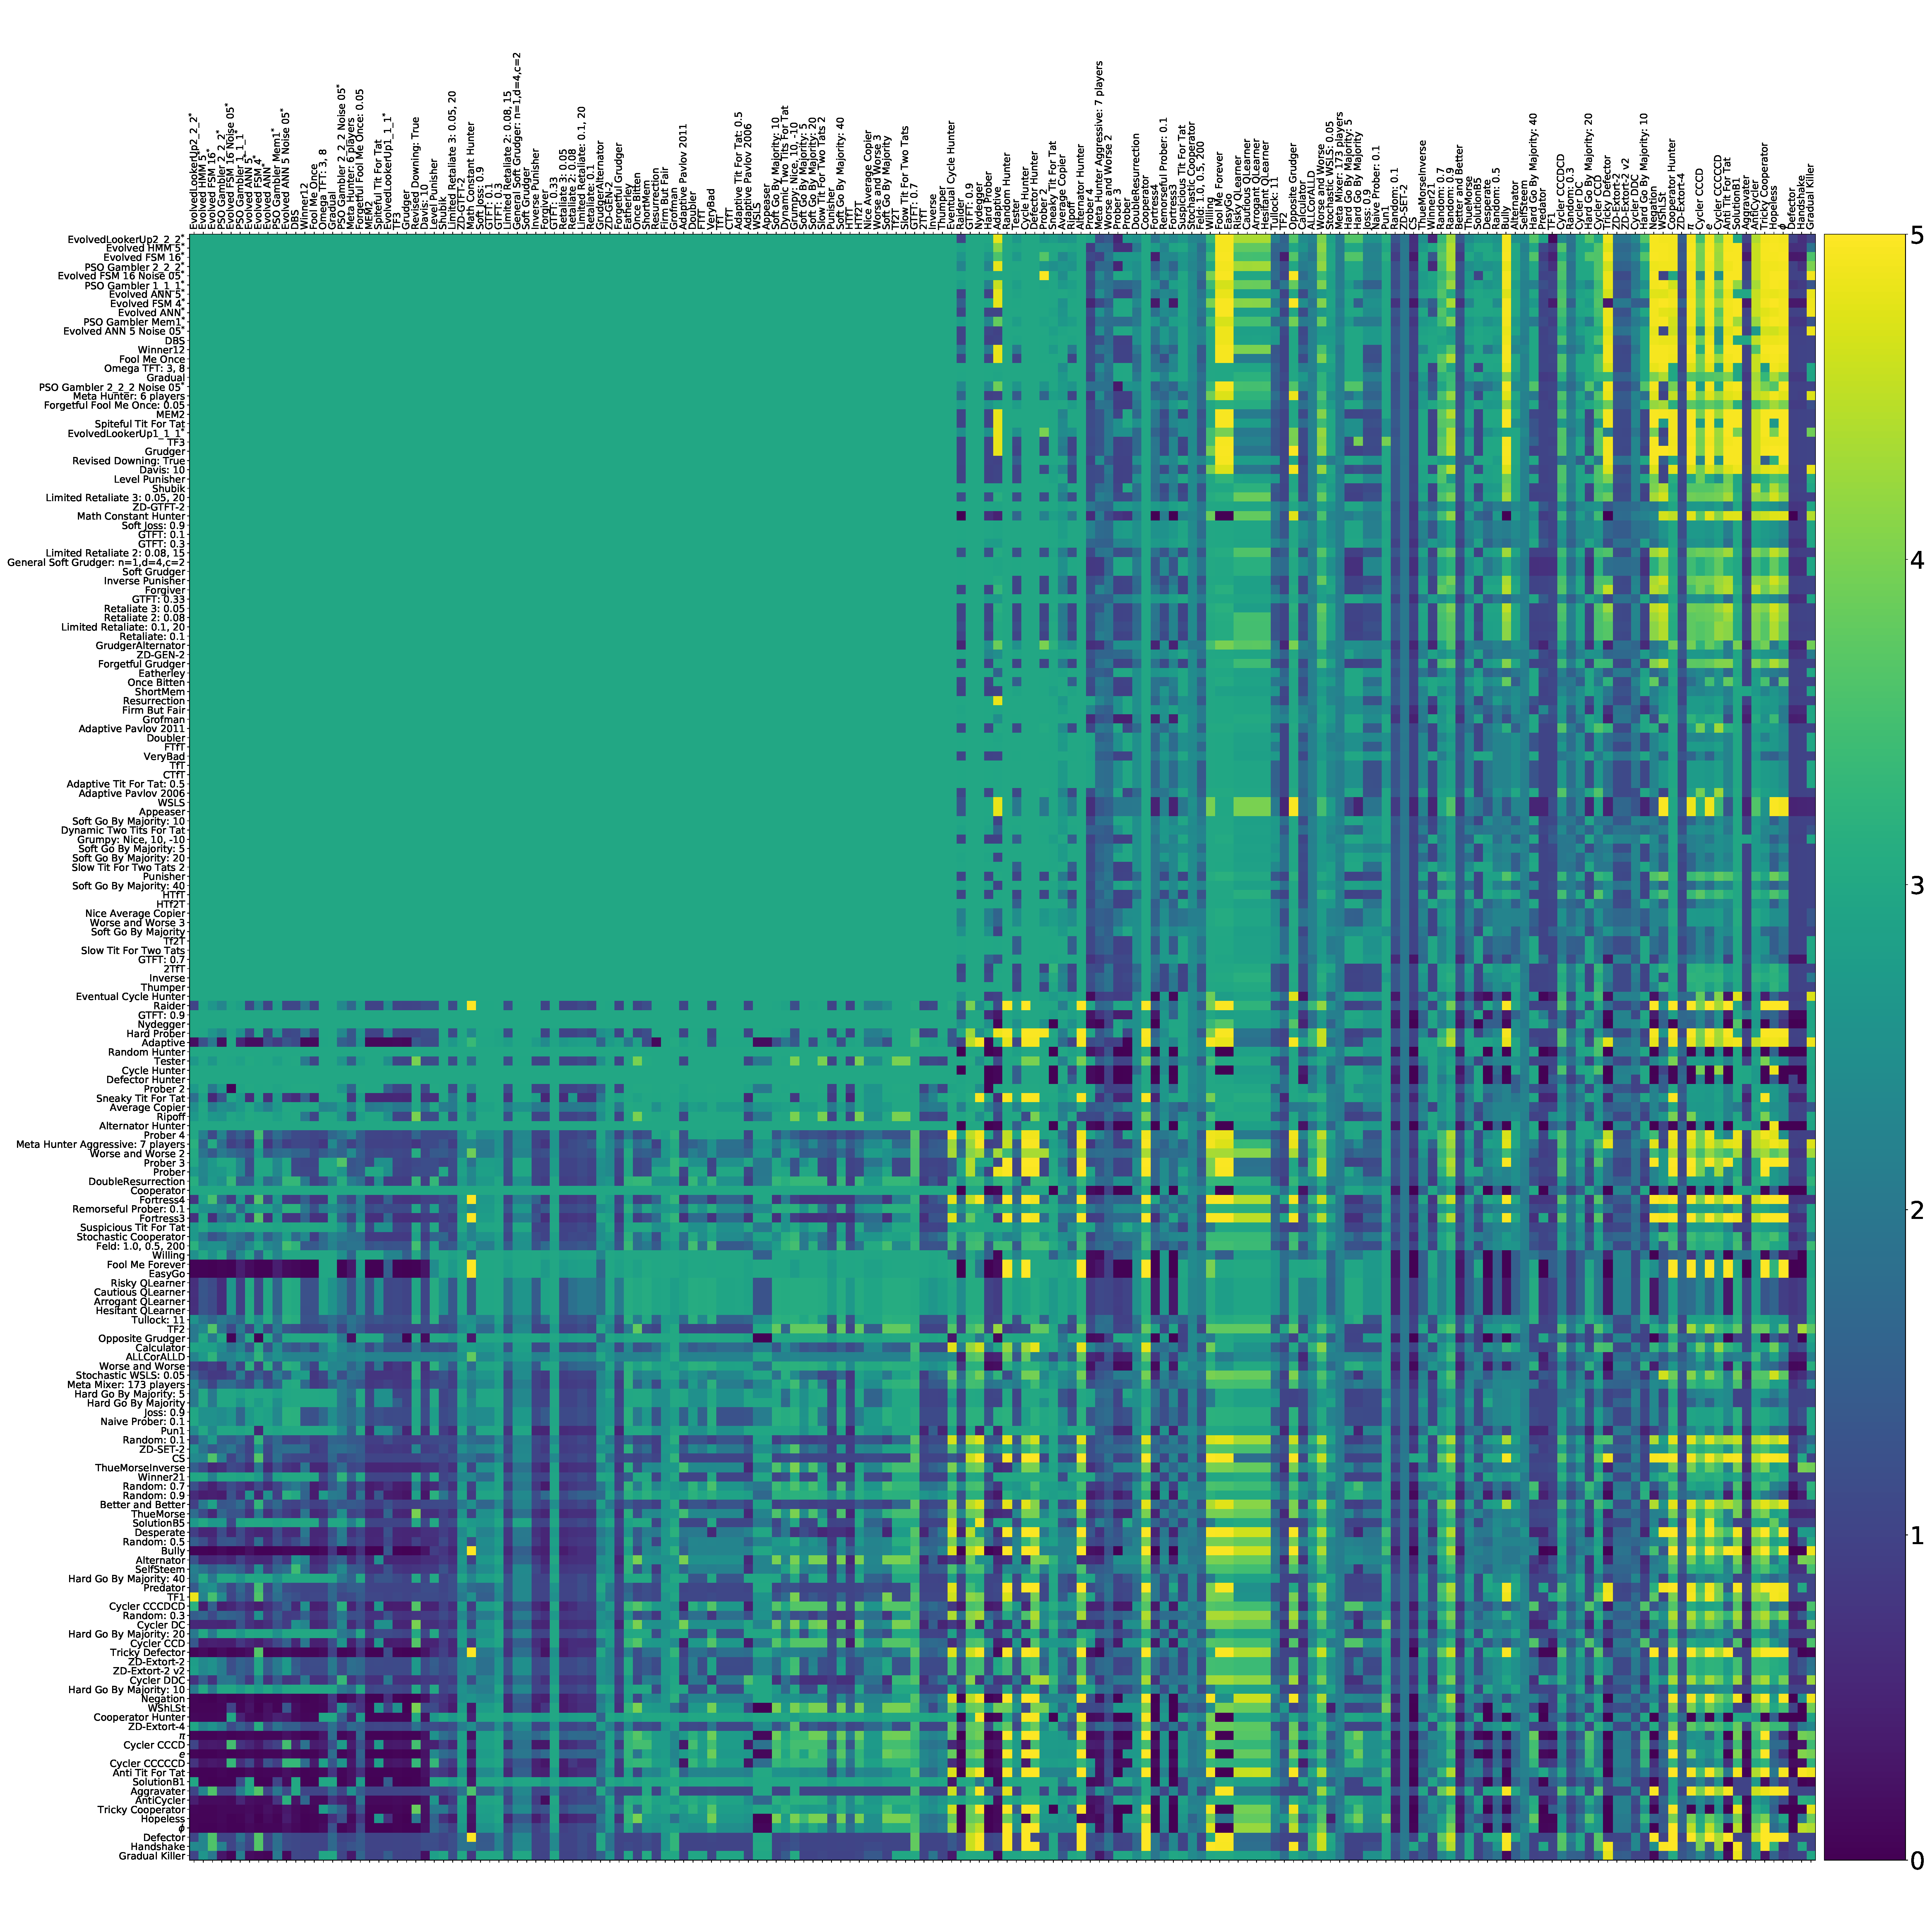
\includegraphics[width=\textwidth]{./assets/standard_scores_heatmap.pdf}
    \caption{Standard Tournament: Mean score per turn of row players against
    column players (ranked by median over
        \protect50000tournaments)}
    \label{fig:standard_heatmap}
\end{figure}

The strategies that win the most matches are Defector, Aggravater, followed by
handshaking and zero determinant strategies. This includes two handshaking
strategies that were the result of training to maximize Moran process fixation.
No strategies were trained specifically to win matches. None of the top scoring
strategies appear in the top 20 list of strategies ranked by match wins.
This can be seen in Figure~\ref{fig:standard_winplot} where the distribution of
the number of wins of each strategy is shown.

\begin{landscape}
    \begin{figure}[!hbtp]
        \centering
        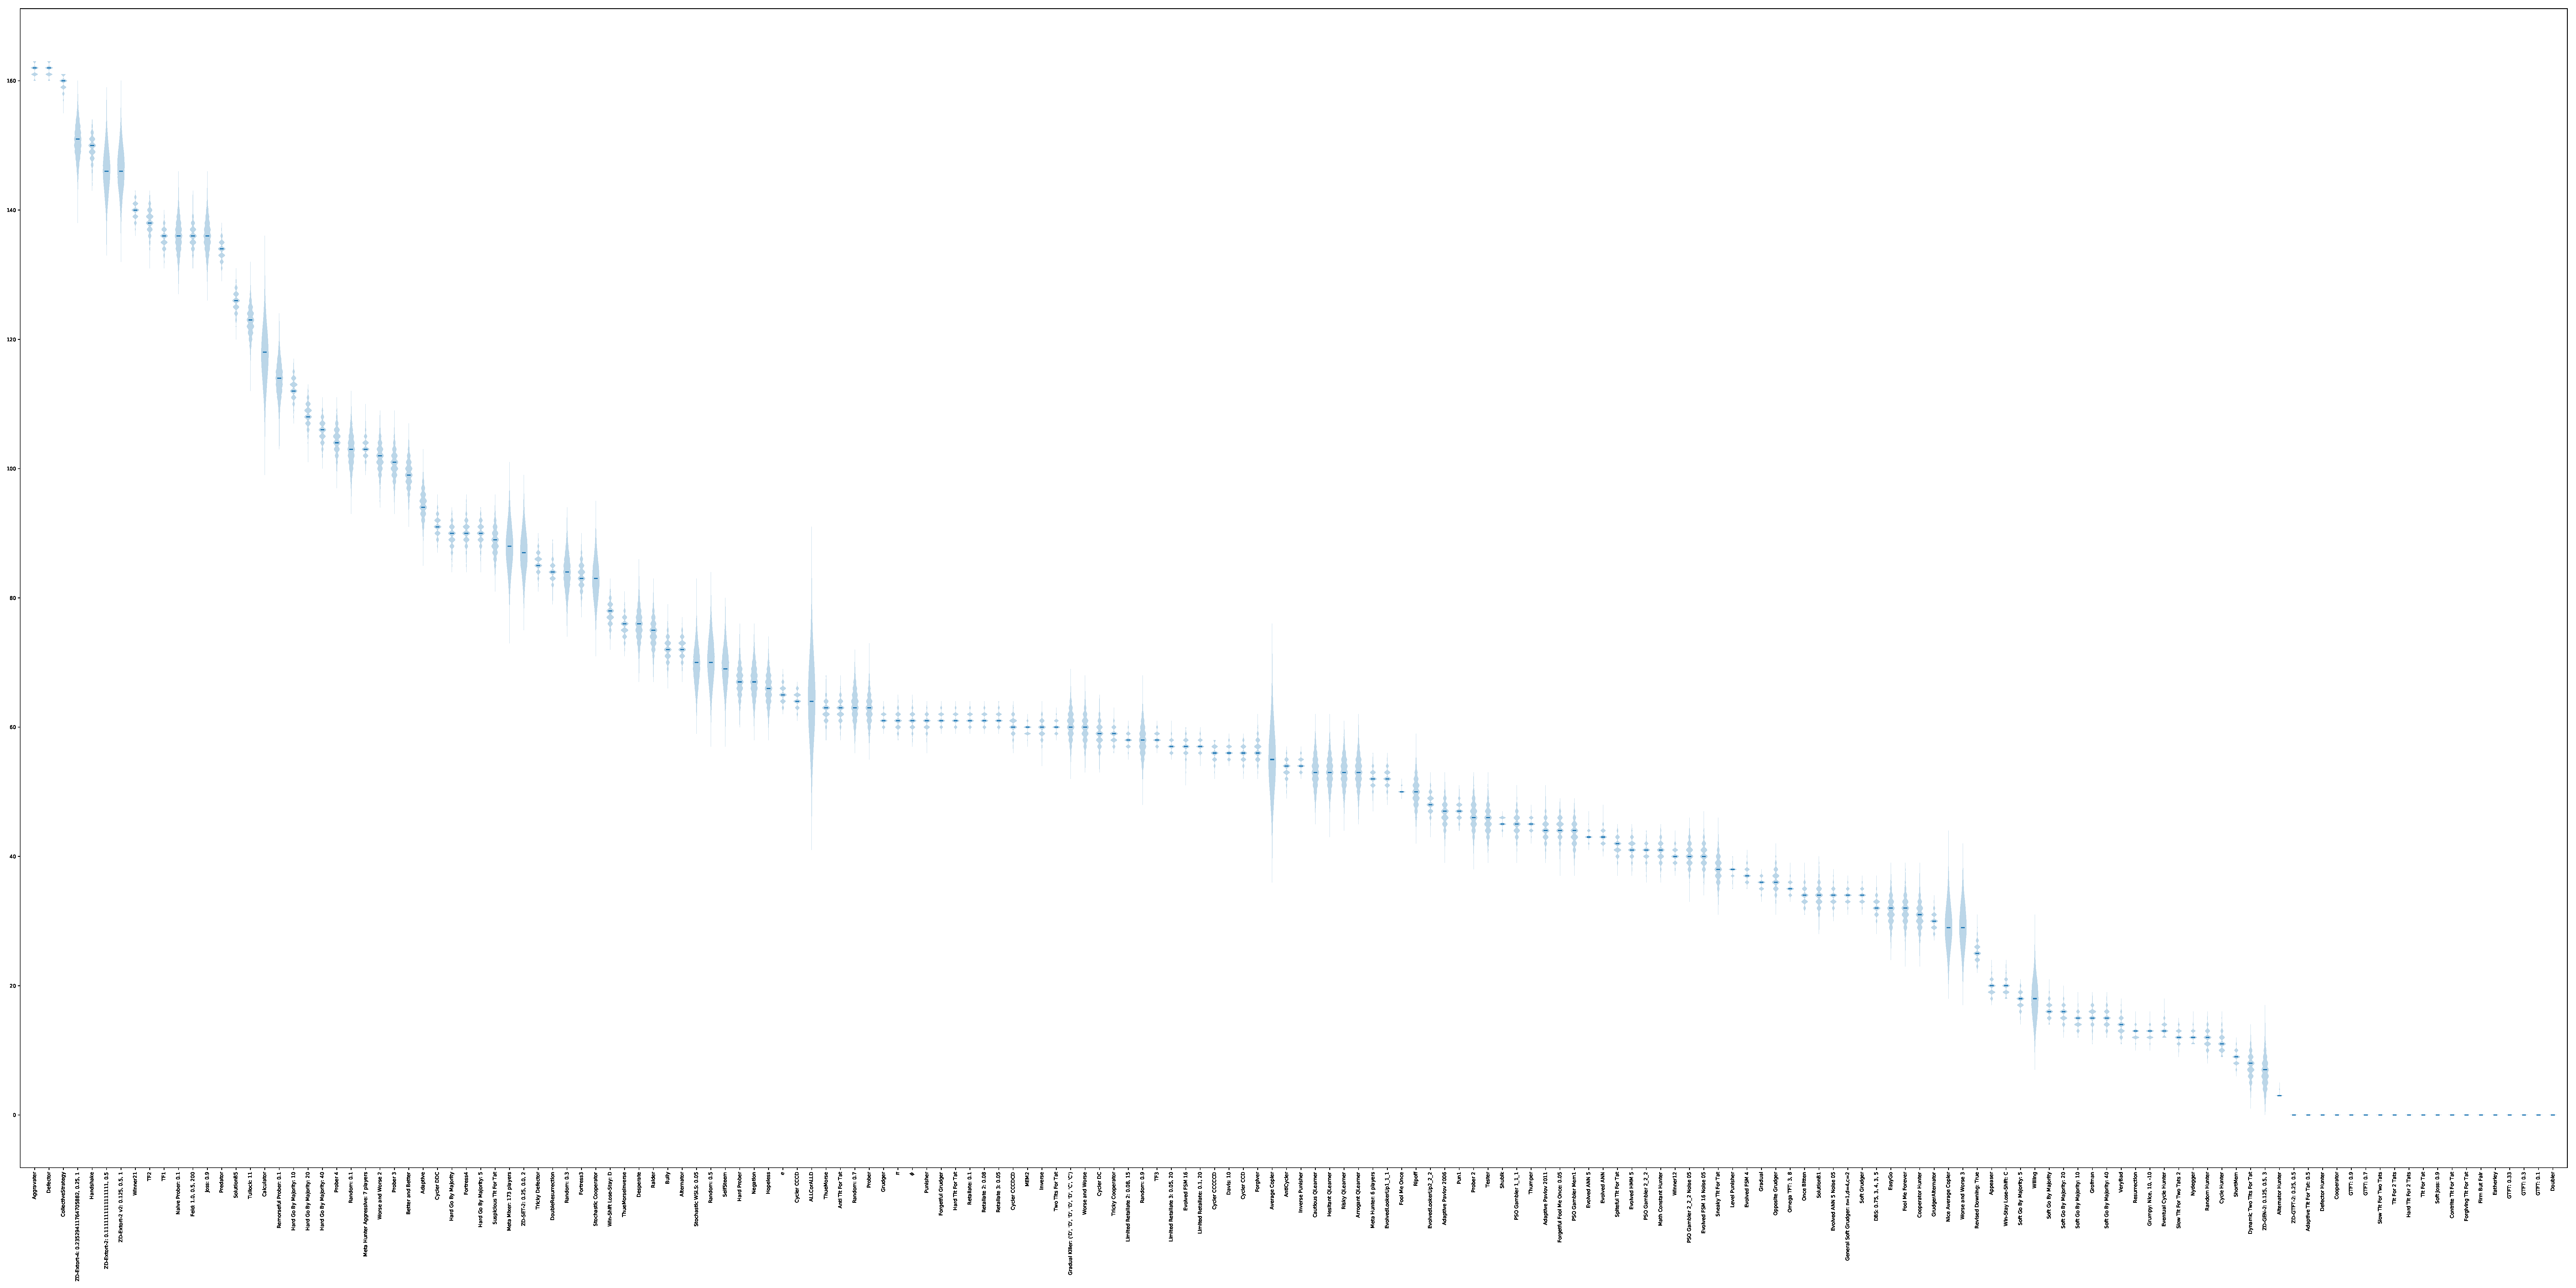
\includegraphics[width=\paperwidth]{./assets/standard_wins_boxplots.pdf}
        \caption{Standard Tournament: number of wins per tournament (ranked by
        median over
        \protect50000tournaments)}
        \label{fig:standard_winplot}
    \end{figure}
\end{landscape}

The number of wins of the top strategies of Table~\ref{tbl:standard_wins} are
shown in Table~\ref{tbl:standard_wins}. It is evident that although these
strategies score highly they do not win many matches: the strategy with the most
number of wins is the Evolved FSM 16 strategy that at most won 60
(\(60/175\approx34\%\)) matches in a given tournament.
% TODO Update this when more data comes in.

\begin{table}[!hbtp]
    \centering
        \begin{tabular}{lrrrrrrrrrr}
\toprule
{} &  count &    mean &    std &  min &    5\% &   25\% &   50\% &   75\% &   95\% &  max \\
\midrule
EvolvedLookerUp2\_2\_2    &  15000 &  48.262 &  1.335 &   43 &  46.0 &  47.0 &  48.0 &  49.0 &  50.0 &   53 \\
Evolved HMM 5           &  15000 &  41.349 &  1.225 &   37 &  39.0 &  41.0 &  41.0 &  42.0 &  43.0 &   45 \\
Evolved FSM 16          &  15000 &  56.973 &  1.102 &   51 &  55.0 &  56.0 &  57.0 &  58.0 &  59.0 &   60 \\
PSO Gambler 2\_2\_2       &  15000 &  40.677 &  1.085 &   36 &  39.0 &  40.0 &  41.0 &  41.0 &  42.0 &   44 \\
Evolved FSM 16 Noise 05 &  15000 &  40.075 &  1.677 &   34 &  37.0 &  39.0 &  40.0 &  41.0 &  43.0 &   47 \\
PSO Gambler 1\_1\_1       &  15000 &  44.980 &  1.597 &   39 &  42.0 &  44.0 &  45.0 &  46.0 &  48.0 &   51 \\
Evolved ANN 5           &  15000 &  43.222 &  0.674 &   41 &  42.0 &  43.0 &  43.0 &  44.0 &  44.0 &   47 \\
Evolved FSM 4           &  15000 &  37.230 &  0.951 &   35 &  36.0 &  37.0 &  37.0 &  38.0 &  39.0 &   41 \\
Evolved ANN             &  15000 &  43.108 &  1.021 &   40 &  42.0 &  42.0 &  43.0 &  44.0 &  45.0 &   48 \\
PSO Gambler Mem1        &  15000 &  43.466 &  1.831 &   37 &  40.0 &  42.0 &  44.0 &  45.0 &  46.0 &   49 \\
Evolved ANN 5 Noise 05  &  15000 &  33.707 &  1.123 &   30 &  32.0 &  33.0 &  34.0 &  34.0 &  35.0 &   38 \\
DBS: 0.75, 3, 4, 3, 5   &  15000 &  32.328 &  1.200 &   28 &  30.0 &  32.0 &  32.0 &  33.0 &  34.0 &   37 \\
Winner12                &  15000 &  40.175 &  1.041 &   37 &  39.0 &  39.0 &  40.0 &  41.0 &  42.0 &   44 \\
Fool Me Once            &  15000 &  50.123 &  0.422 &   49 &  50.0 &  50.0 &  50.0 &  50.0 &  51.0 &   52 \\
Omega TFT: 3, 8         &  15000 &  35.158 &  0.860 &   33 &  34.0 &  35.0 &  35.0 &  36.0 &  37.0 &   39 \\
\bottomrule
\end{tabular}

        \caption{Standard Tournament: Number of wins per tournament
        of top 15 strategies (ranked by median score over
        \protect50000tournaments)}
        \label{tbl:standard_wins}
\end{table}

Finally, Table~\ref{tbl:standard_ranks} and
Figure~\ref{fig:standard_ranks_boxplot} show the ranks (based on median score)
of each strategy over the repeated tournaments. Whilst there is some
stochasticity, the top three strategies almost always rank in the top three. For
example, the worst that the Evolved Lookerup 2 2 2 ranks in a given tournament
is 8th.


\begin{table}[!hbtp]
    \centering
        \begin{tabular}{lrrrrrrrrr}
\toprule
{} &    mean &    std &  min &    5\% &   25\% &   50\% &   75\% &   95\% &  max \\
\midrule
EvolvedLookerUp2\_2\_2$^{*}$    &   2.171 &  1.069 &    1 &   1.0 &   1.0 &   2.0 &   3.0 &   4.0 &    8 \\
Evolved HMM 5$^{*}$           &   2.325 &  1.275 &    1 &   1.0 &   1.0 &   2.0 &   3.0 &   5.0 &   10 \\
Evolved FSM 16$^{*}$          &   2.488 &  1.299 &    1 &   1.0 &   1.0 &   2.0 &   3.0 &   5.0 &   10 \\
PSO Gambler 2\_2\_2$^{*}$       &   3.961 &  1.527 &    1 &   2.0 &   3.0 &   4.0 &   5.0 &   7.0 &   10 \\
Evolved FSM 16 Noise 05$^{*}$ &   6.298 &  1.688 &    1 &   4.0 &   5.0 &   6.0 &   7.0 &   9.0 &   11 \\
PSO Gambler 1\_1\_1$^{*}$       &   7.091 &  2.504 &    1 &   3.0 &   5.0 &   7.0 &   9.0 &  10.0 &   17 \\
Evolved ANN 5$^{*}$           &   7.285 &  1.524 &    2 &   5.0 &   6.0 &   7.0 &   8.0 &  10.0 &   11 \\
Evolved FSM 4$^{*}$           &   7.521 &  1.630 &    2 &   5.0 &   6.0 &   8.0 &   9.0 &  10.0 &   12 \\
Evolved ANN$^{*}$             &   7.899 &  1.450 &    2 &   5.0 &   7.0 &   8.0 &   9.0 &  10.0 &   12 \\
PSO Gambler Mem1$^{*}$        &   8.223 &  2.534 &    1 &   4.0 &   6.0 &   9.0 &  10.0 &  12.0 &   20 \\
Evolved ANN 5 Noise 05$^{*}$  &  11.362 &  0.872 &    8 &  10.0 &  11.0 &  11.0 &  12.0 &  13.0 &   16 \\
DBS                           &  12.191 &  1.121 &    9 &  11.0 &  11.0 &  12.0 &  13.0 &  14.0 &   16 \\
Winner12                      &  13.224 &  1.136 &    9 &  11.0 &  12.0 &  13.0 &  14.0 &  15.0 &   17 \\
Fool Me Once                  &  13.961 &  1.080 &    9 &  12.0 &  13.0 &  14.0 &  15.0 &  15.0 &   17 \\
Omega TFT: 3, 8               &  14.274 &  1.300 &    9 &  12.0 &  13.0 &  15.0 &  15.0 &  16.0 &   19 \\
\bottomrule
\end{tabular}

        \caption{Standard Tournament: Rank in each tournament
        of top 15 strategies (ranked by median over
        \protect50000tournaments)}
        \label{tbl:standard_ranks}
\end{table}

\begin{landscape}
    \begin{figure}[!hbtp]
        \centering
        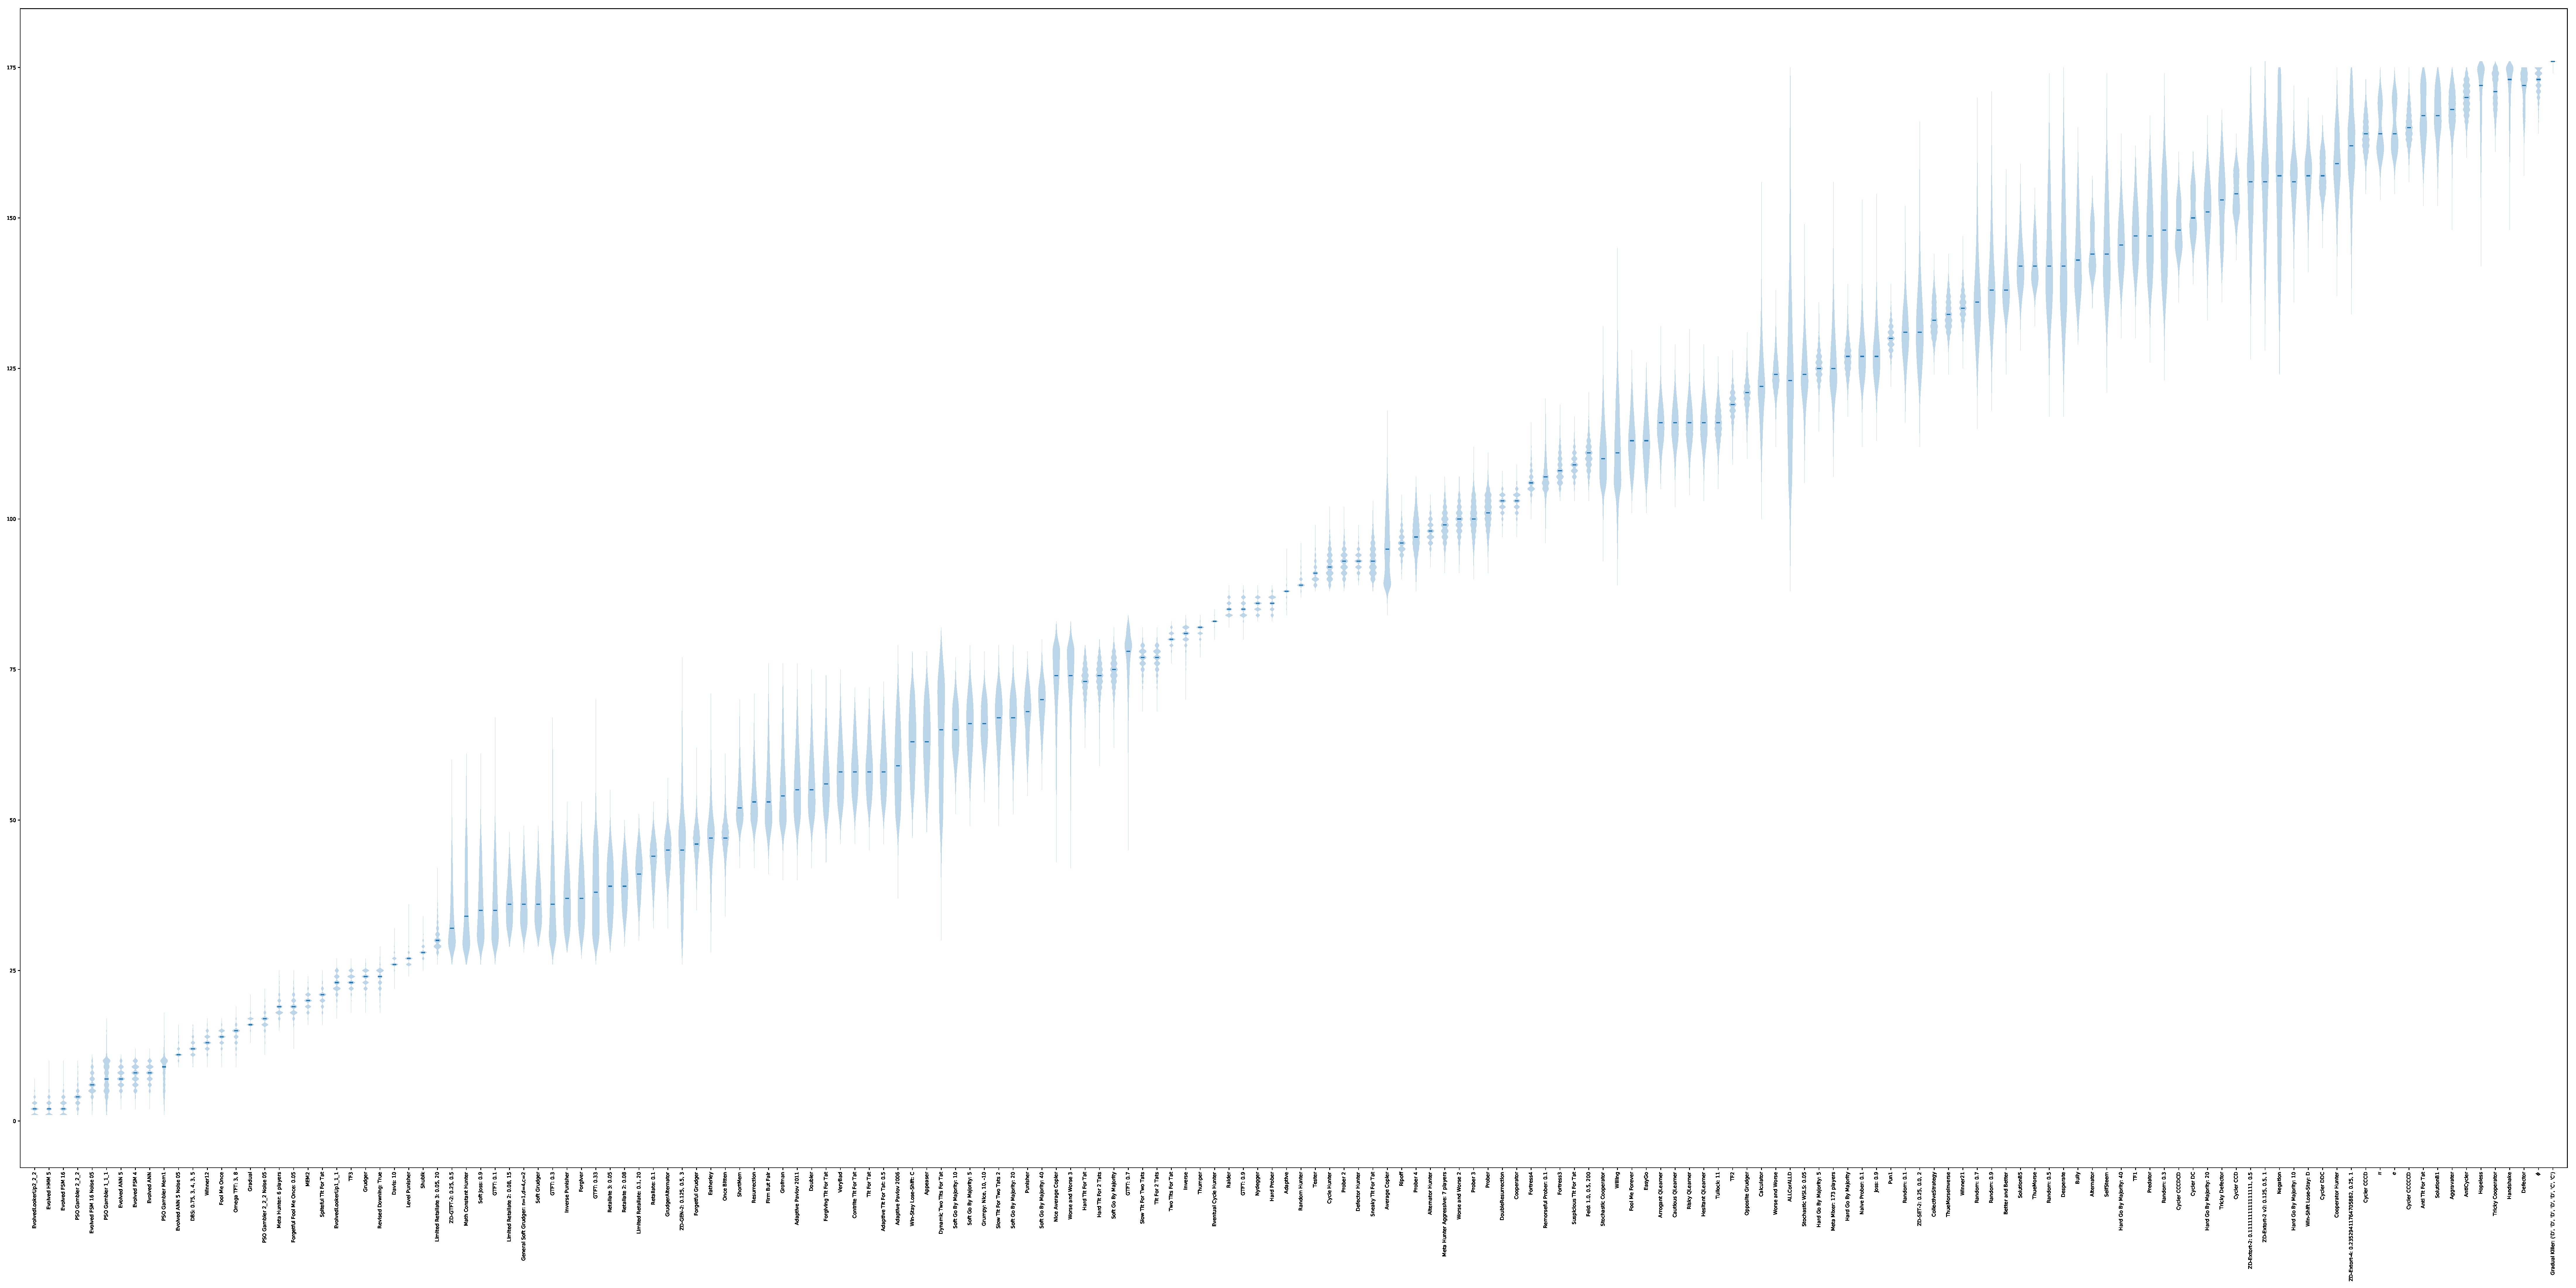
\includegraphics[width=\paperwidth]{./assets/standard_ranks_boxplots.pdf}
        \caption{Standard Tournament: rank in each tournament (ranked by
        median over
        \protect50000tournaments)}
        \label{fig:standard_ranks_boxplot}
    \end{figure}
\end{landscape}


Using the method of fingerprinting described in \cite{ashlock2008fingerprinting}
% TODO This is actually a numerical approximation of the fingerprinting
% described in ashlock's paper. There they consider a fingerprint to be an
% analytic function.
\cite{ashlock2009fingerprint}, we can compare
strategies. For the top performing noisy strategies there is a striking similarity
in the fingerprints.

\begin{figure}[!hbtp]
    \centering
    \begin{subfigure}[t]{.3\textwidth}
        \centering
        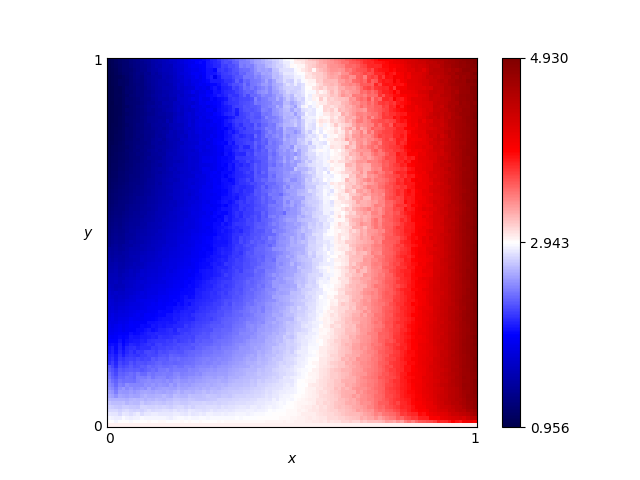
\includegraphics[width=\textwidth]{./assets/EvolvedLookerUp2_2_2.png}
        \caption{Fingerprint for EvolvedLookerUp\_2\_2\_2}
    \end{subfigure}%
    ~
    \begin{subfigure}[t]{.3\textwidth}
        \centering
        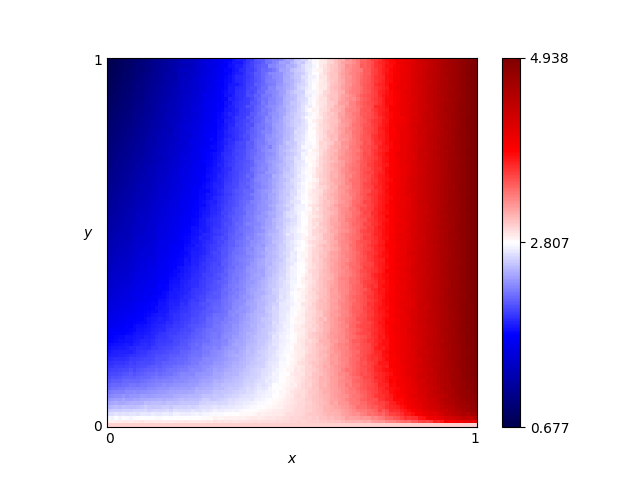
\includegraphics[width=\textwidth]{./assets/Evolved_HMM_5.png}
        \caption{Fingerprint for Evolved\_HMM\_5}
    \end{subfigure}%
    ~
    \begin{subfigure}[t]{.3\textwidth}
        \centering
        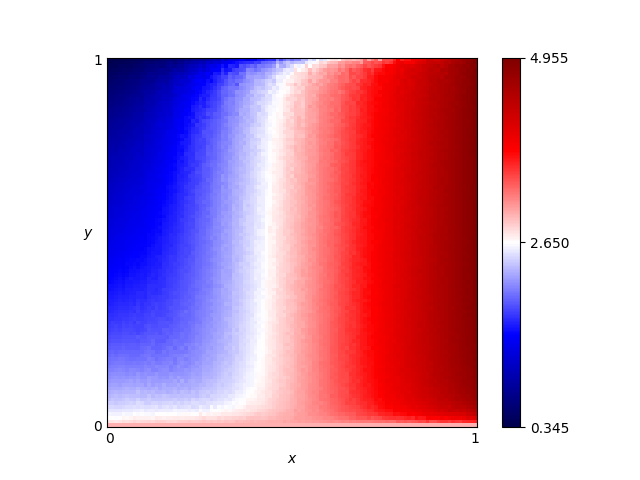
\includegraphics[width=\textwidth]{./assets/Evolved_FSM_16.png}
        \caption{Fingerprint for Evolved\_FSM\_16}
    \end{subfigure}%

    \caption{Comparison of Fingerprints for Noisy Tournament Top 3}
    \label{fig:comparison_fingerprint_noisy}
\end{figure}


\subsection{Noisy Tournament}

We also ran noisy tournaments in which there is a 5\% chance that an action is
flipped. As shown in Table~\ref{tbl:noisy_score} and
Figure~\ref{fig:noisy_score}, the best performing strategies in median payoff
are DBS, designed to correct for noise, followed by two strategies trained in
the presence of noise and three trained strategies trained without noise. One of
the strategies trained with noise (PSO Gambler) actually performs less well than
some of the other high ranking strategies including
Spiteful TFT (TFT but defects indefinitely if the opponent defects twice
consecutively) and OmegaTFT (also designed to handle noise).

% Table of best strategies
\begin{table}[!hbtp]
    \centering
        \begin{tabular}{lrrrrrrrrr}
\toprule
{} &   mean &    std &    min &     5\% &    25\% &    50\% &    75\% &    95\% &    max \\
\midrule
DBS: 0.75, 3, 4, 3, 5      &  2.573 &  0.024 &  2.483 &  2.533 &  2.556 &  2.573 &  2.589 &  2.613 &  2.667 \\
Evolved ANN 5 Noise 05     &  2.534 &  0.025 &  2.418 &  2.492 &  2.517 &  2.534 &  2.551 &  2.575 &  2.629 \\
Evolved FSM 16 Noise 05    &  2.515 &  0.031 &  2.374 &  2.464 &  2.494 &  2.515 &  2.536 &  2.566 &  2.642 \\
Evolved ANN 5              &  2.409 &  0.030 &  2.297 &  2.359 &  2.389 &  2.409 &  2.430 &  2.459 &  2.536 \\
Evolved FSM 4              &  2.393 &  0.027 &  2.286 &  2.349 &  2.374 &  2.393 &  2.411 &  2.437 &  2.493 \\
Evolved HMM 5              &  2.392 &  0.026 &  2.291 &  2.349 &  2.374 &  2.392 &  2.409 &  2.435 &  2.492 \\
Level Punisher             &  2.389 &  0.025 &  2.290 &  2.347 &  2.372 &  2.389 &  2.406 &  2.429 &  2.487 \\
Omega TFT: 3, 8            &  2.387 &  0.026 &  2.270 &  2.343 &  2.369 &  2.387 &  2.404 &  2.429 &  2.490 \\
Spiteful Tit For Tat       &  2.383 &  0.030 &  2.259 &  2.334 &  2.363 &  2.383 &  2.403 &  2.432 &  2.488 \\
Evolved FSM 16             &  2.375 &  0.029 &  2.256 &  2.326 &  2.355 &  2.375 &  2.395 &  2.423 &  2.494 \\
PSO Gambler 2\_2\_2 Noise 05 &  2.371 &  0.029 &  2.258 &  2.324 &  2.352 &  2.371 &  2.390 &  2.417 &  2.477 \\
Adaptive                   &  2.369 &  0.038 &  2.217 &  2.307 &  2.344 &  2.369 &  2.394 &  2.432 &  2.510 \\
Evolved ANN                &  2.365 &  0.022 &  2.280 &  2.329 &  2.351 &  2.365 &  2.380 &  2.401 &  2.483 \\
Math Constant Hunter       &  2.344 &  0.023 &  2.263 &  2.308 &  2.329 &  2.344 &  2.359 &  2.382 &  2.431 \\
Gradual                    &  2.341 &  0.021 &  2.248 &  2.306 &  2.326 &  2.341 &  2.355 &  2.375 &  2.429 \\
\bottomrule
\end{tabular}

        \caption{Noisy (5\%) Tournament: Mean score per turn of top 15 strategies
        (ranked by median over
        \protect50000tournaments)
        ~$^{*}$ indicates that the strategy was trained.}
        \label{tbl:noisy_score}
\end{table}


\begin{landscape}
    \begin{figure}[!hbtp]
        \centering
        \includegraphics[width=\paperwidth]{./assets/noisy_scores_boxplots.pdf}
        \caption{Noisy (5\%) Tournament: Mean score per turn (ranked by median
        over
        \protect50000tournaments)}
        \label{fig:noisy_score}
    \end{figure}
\end{landscape}


The strategies trained in the presence of noise are also among the best
performers in the absence of noise. As shown in Figure~\ref{fig:noisy_heatmap}
the cluster of mutually cooperative strategies is broken by the noise at 5\%. A
similar collection of players excels at winning matches but again they have a
poor total payoff.

\begin{figure}[!hbtp]
    \centering
    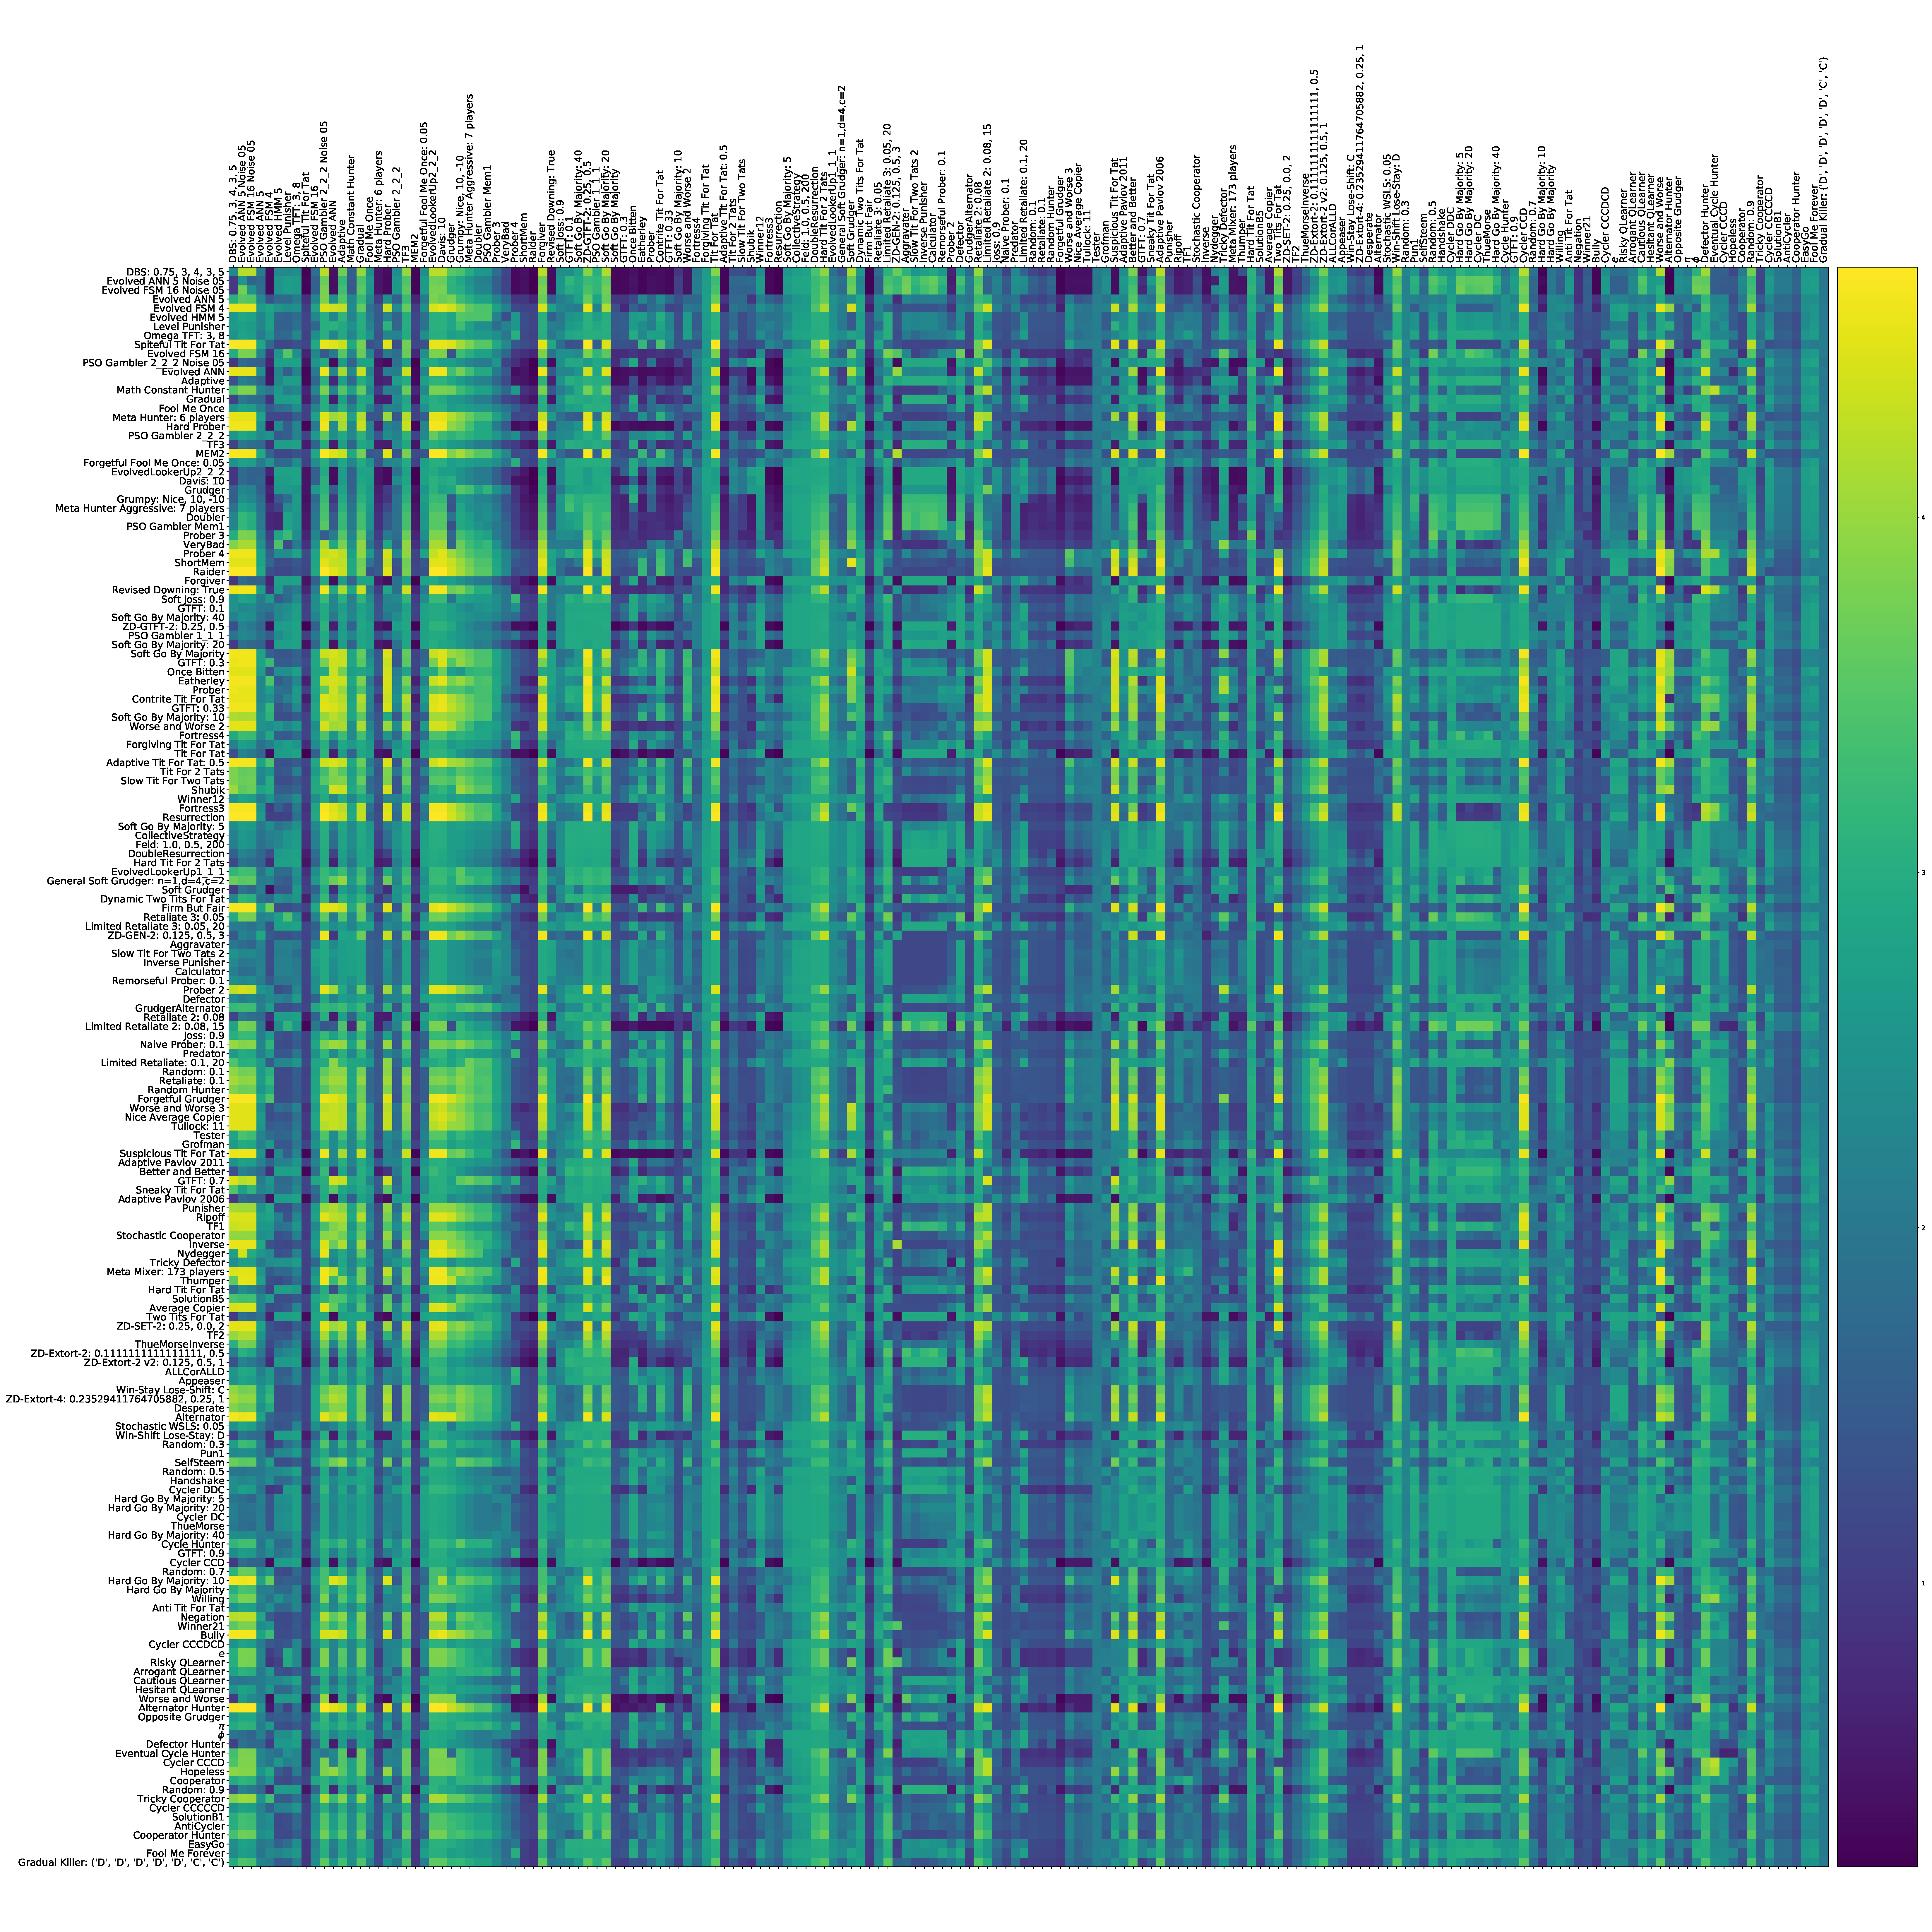
\includegraphics[width=\textwidth]{./assets/noisy_scores_heatmap.pdf}
    \caption{Noisy (5\%) Tournament: Mean score per turn of row players against
    column players (ranked by median over
        \protect50000tournaments)}
    \label{fig:noisy_heatmap}
\end{figure}

As shown in Figure~\ref{fig:noisy_winplot} the strategies tallying the most wins
are somewhat similar, with Defector, the handshaking CollectiveStrategy, and
Aggravate appearing as the top three again.

\begin{landscape}
    \begin{figure}[!hbtp]
        \centering
        \includegraphics[width=\paperwidth]{./assets/noisy_wins_boxplots.pdf}
        \caption{Noisy (5\%) Tournament: number of wins per tournament (ranked by
        median over
        \protect50000tournaments)}
        \label{fig:noisy_winplot}
    \end{figure}
\end{landscape}

As shown in Table~\ref{tbl:noisy_wins}, the top ranking strategies win a larger
number of matches in the presence of noise. For example Spiteful Tit For Tat in
one tournament won almost all its matches (167).

\begin{table}[!hbtp]
    \centering
        \begin{tabular}{lrrrrrrrrr}
\toprule
{} &     mean &    std &  min &     5\% &    25\% &    50\% &    75\% &    95\% &  max \\
\midrule
DBS                              &  102.545 &  3.671 &   87 &   97.0 &  100.0 &  103.0 &  105.0 &  109.0 &  118 \\
Evolved ANN 5 Noise 05$^{*}$     &   75.026 &  4.226 &   57 &   68.0 &   72.0 &   75.0 &   78.0 &   82.0 &   93 \\
Evolved FSM 16 Noise 05$^{*}$    &   88.699 &  3.864 &   74 &   82.0 &   86.0 &   89.0 &   91.0 &   95.0 &  104 \\
Evolved ANN 5$^{*}$              &  137.878 &  4.350 &  118 &  131.0 &  135.0 &  138.0 &  141.0 &  145.0 &  156 \\
Evolved FSM 4$^{*}$              &   74.250 &  2.694 &   64 &   70.0 &   72.0 &   74.0 &   76.0 &   79.0 &   85 \\
Evolved HMM 5$^{*}$              &   88.189 &  2.774 &   77 &   84.0 &   86.0 &   88.0 &   90.0 &   93.0 &   99 \\
Level Punisher                   &   94.263 &  4.789 &   75 &   86.0 &   91.0 &   94.0 &   97.0 &  102.0 &  116 \\
Omega TFT: 3, 8                  &  131.655 &  4.302 &  112 &  125.0 &  129.0 &  132.0 &  135.0 &  139.0 &  150 \\
Spiteful Tit For Tat             &  155.030 &  3.326 &  133 &  150.0 &  153.0 &  155.0 &  157.0 &  160.0 &  167 \\
Evolved FSM 16$^{*}$             &  103.288 &  3.631 &   89 &   97.0 &  101.0 &  103.0 &  106.0 &  109.0 &  118 \\
PSO Gambler 2\_2\_2 Noise 05$^{*}$ &   90.515 &  4.012 &   75 &   84.0 &   88.0 &   90.0 &   93.0 &   97.0 &  109 \\
Adaptive                         &  101.898 &  4.899 &   83 &   94.0 &   99.0 &  102.0 &  105.0 &  110.0 &  124 \\
Evolved ANN$^{*}$                &  138.514 &  3.401 &  125 &  133.0 &  136.0 &  139.0 &  141.0 &  144.0 &  153 \\
Math Constant Hunter             &   93.010 &  3.254 &   79 &   88.0 &   91.0 &   93.0 &   95.0 &   98.0 &  107 \\
Gradual                          &  101.899 &  2.870 &   91 &   97.0 &  100.0 &  102.0 &  104.0 &  107.0 &  114 \\
\bottomrule
\end{tabular}

        \caption{Noisy (5\%) Tournament: Number of wins per tournament
        of top 15 strategies (ranked by median score over
        \protect50000tournaments)}
        \label{tbl:noisy_wins}
\end{table}


Finally, Table~\ref{tbl:noisy_ranks} and
Figure~\ref{fig:noisy_ranks_boxplot} show the ranks (based on median score)
of each strategy over the repeated tournaments. We see that the stochasticity
of the ranks understandably increases the DBS strategy never ranks lower than
second and wins 75\% of the time. The two strategies trained for noisy
tournaments rank in the top three 95\% of the time.
% TODO Possibly update this with more data.

\begin{table}[!hbtp]
    \centering
        \begin{tabular}{lrrrrrrrrr}
\toprule
{} &    mean &    std &  min &      5\% &   25\% &   50\% &   75\% &   95\% &  max \\
\midrule
DBS                              &   1.205 &  0.468 &    1 &   1.000 &   1.0 &   1.0 &   1.0 &   2.0 &    3 \\
Evolved ANN 5 Noise 05$^{*}$     &   2.184 &  0.629 &    1 &   1.000 &   2.0 &   2.0 &   3.0 &   3.0 &    5 \\
Evolved FSM 16 Noise 05$^{*}$    &   2.626 &  0.618 &    1 &   1.000 &   2.0 &   3.0 &   3.0 &   3.0 &    9 \\
Evolved ANN 5$^{*}$              &   6.371 &  2.786 &    2 &   4.000 &   4.0 &   5.0 &   8.0 &  12.0 &   31 \\
Evolved FSM 4$^{*}$              &   7.919 &  3.175 &    3 &   4.000 &   5.0 &   7.0 &  10.0 &  14.0 &   33 \\
Evolved HMM 5$^{*}$              &   7.996 &  3.110 &    3 &   4.000 &   6.0 &   7.0 &  10.0 &  14.0 &   26 \\
Level Punisher                   &   8.337 &  3.083 &    3 &   4.000 &   6.0 &   8.0 &  10.0 &  14.0 &   26 \\
Omega TFT: 3, 8                  &   8.510 &  3.249 &    3 &   4.000 &   6.0 &   8.0 &  11.0 &  14.0 &   32 \\
Spiteful Tit For Tat             &   9.159 &  3.772 &    3 &   4.000 &   6.0 &   9.0 &  12.0 &  16.0 &   40 \\
Evolved FSM 16$^{*}$             &  10.218 &  4.099 &    3 &   4.975 &   7.0 &  10.0 &  13.0 &  17.0 &   56 \\
PSO Gambler 2\_2\_2 Noise 05$^{*}$ &  10.760 &  4.102 &    3 &   5.000 &   8.0 &  10.0 &  13.0 &  18.0 &   47 \\
Evolved ANN$^{*}$                &  11.346 &  3.252 &    3 &   6.000 &   9.0 &  11.0 &  13.0 &  17.0 &   32 \\
Adaptive                         &  11.420 &  5.739 &    3 &   4.000 &   7.0 &  11.0 &  14.0 &  21.0 &   63 \\
Math Constant Hunter             &  14.668 &  3.788 &    3 &   9.000 &  12.0 &  15.0 &  17.0 &  21.0 &   43 \\
Gradual                          &  15.163 &  3.672 &    4 &  10.000 &  13.0 &  15.0 &  17.0 &  21.0 &   49 \\
\bottomrule
\end{tabular}

        \caption{Noisy (5\%) Tournament: Rank in each tournament
        of top 15 strategies (ranked by median over
        \protect50000tournaments)}
        \label{tbl:noisy_ranks}
\end{table}

\begin{landscape}
    \begin{figure}[!hbtp]
        \centering
        \includegraphics[width=\paperwidth]{./assets/noisy_ranks_boxplots.pdf}
        \caption{Noisy (5\%) Tournament: rank in each tournament (ranked by
        median over
        \protect50000tournaments)}
        \label{fig:noisy_ranks_boxplot}
    \end{figure}
\end{landscape}

Again we compare the fingerprints. For the top performing noisy strategies there
is a striking similarity in the fingerprints which indicates that the strategies
may behave similarly in principle.

\begin{figure}[!hbtp]
    \centering
    \begin{subfigure}[t]{.3\textwidth}
        \centering
        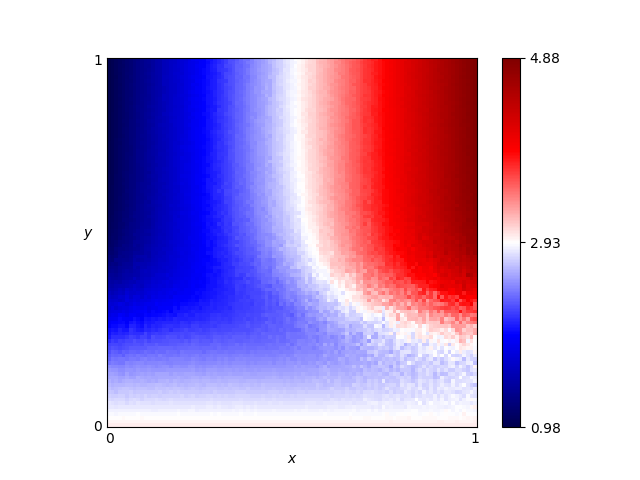
\includegraphics[width=\textwidth]{./assets/DBS.png}
        \caption{Fingerprint for DBS}
    \end{subfigure}%
    ~
    \begin{subfigure}[t]{.3\textwidth}
        \centering
        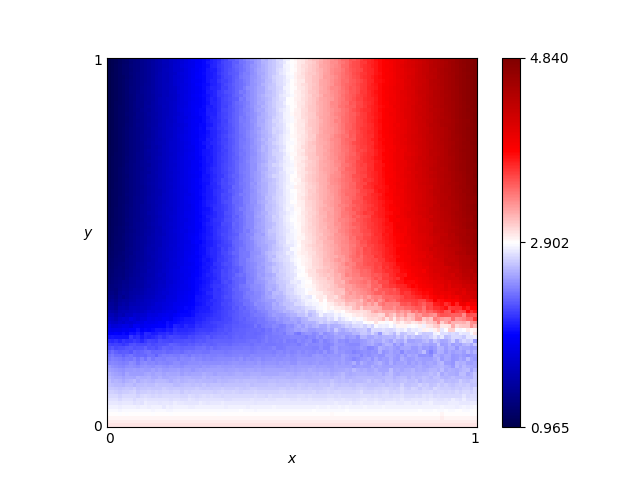
\includegraphics[width=\textwidth]{./assets/Evolved_ANN_5_Noise_05.png}
        \caption{Fingerprint for Evolved\_ANN\_5\_Noise\_05}
    \end{subfigure}%
    ~
    \begin{subfigure}[t]{.3\textwidth}
        \centering
        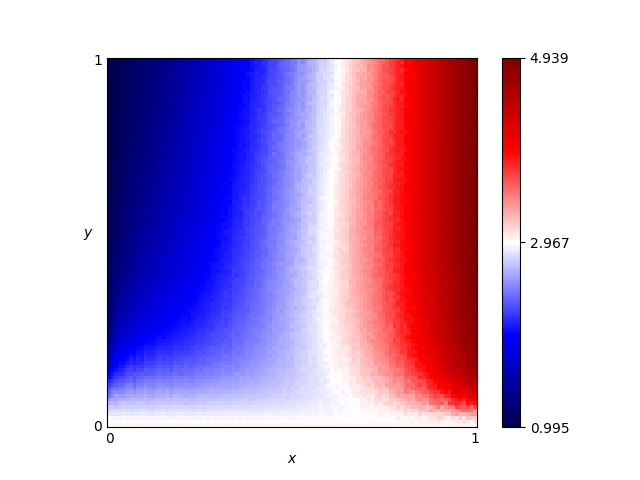
\includegraphics[width=\textwidth]{./assets/Evolved_FSM_16_Noise_05.png}
        \caption{Fingerprint for Evolved\_FSM\_16\_Noise\_05}
    \end{subfigure}%

    \caption{Comparison of Fingerprints for Noisy Tournament Top 3}
    \label{fig:comparison_fingerprint_noisy}
\end{figure}


\section{Methods}

We trained a variety of strategies using evolutionary algorithms, and in the
case of PSO Gambler using a particle swarm algorithm. The evolutionary algorithms
used standard techniques, varying strategies by mutation and crossover, and
evaluating the performance against each opponent for many repetitions. The
best performing strategies in each generation are persisted, variants created,
and objective functions computed again. This process continues for approximately
200 generations or until strategies no longer improve significantly.

% TODO: Diagram with ANN training performance?

All training code is available on github. There are objective functions for
\begin{itemize}
 \item total or mean payoff
 \item total or mean payoff difference (unused in this work)
 \item total Moran process wins (fixation probability)
\end{itemize}

These objectives can be easily modified to suit other purposes. New strategies
can be easily trained with variations including noise, spatial structure, and
probabilistically ending matches.

\section{Discussion}

The tournament results indicate that pre-trained strategies are generally better
than human designed strategies at maximizing payoff against a diverse set of
opponents. A simple evolutionary algorithm produces strategies based on multiple
standard machine learning techniques that are able to achieve a higher average
score than any other known opponent in a standard tournament. Most of the trained
strategies use multiple rounds of the history of play (some using all of it) and
outperform memory-one strategies (though the trained memory one strategy performs
well). The generic structure of the trained strategies did not appear to be
critical -- strategies based on lookup tables, finite state machines, and stochastic
variants all performed well. Single layer neural networks also performed well
though these had some aspect of human involvement in the selection of features.
The success of the other strategy types suggests that a deeper network that
incorporates feature engineering would likely also perform well.

In opposition to historical tournament results and community folklore,
our results show that complex strategies can be very effective for the
IPD. It is not the complexity of strategies that is disadvantageous; rather that directly
designing a broadly effective strategy is no easy task. Of all the human-designed
strategies in the library, only DBS consistently performs well, and it is
substantially more complex than traditional tournament winners like TFT, OmegaTFT,
and zero determinant strategies. Furthermore, dealing with noise is difficult
for most strategies. Two strategies designed specifically to account for noise,
DBS and OmegaTFT, perform well and only DBS performs better than our trained
strategies.

Of the strategies trained to maximize their median score all are generally
cooperative, not defecting until the opponent defects. Maximizing for individual
performance across a collection of opponents leads to mutual cooperation despite
the fact that mutual cooperation is an unstable evolutionary equilibrium for the prisoner's
dilemma. Specifically we note that the reinforcement learning process for maximizing
payout does not lead to exploitative zero determinant strategies, which may also
be a result of the collection of training strategies, of which several retaliate harshly.

We take the liberty of generalizing from the results of this study. For the trained
strategies utilizing look up tables we generally found those that incorporate
one of more of the initial rounds of play outperformed those that did not. The
strategies based on neural networks and finite state machines also are able to
condition throughout a match on the first rounds of play. Accordingly, we conclude
that first impressions matter in the IPD\@. The best strategies are nice (never
defecting first) and this property could be further investigated with the library
in future work by e.g. forcing all strategies to defect on the first round.


Finally, we note that as the library grows, the top performing strategies
sometimes shuffle, and are not retrained regularly. Most of the strategies were
trained on an earlier version of the library (v2.2.0) that did not include DBS
and several other opponents. The precise parameters that are optimal will depend
on the pool of opponents. Moreover we have not extensively trained strategies to
determine the minimum parameters that are sufficient -- neural networks with
fewer nodes and features and finite state machines with fewer states may suffice.
See \cite{ashlock2013impact} for discussion of resource availability for IPD
strategies. It may be possible to train strategies more effective in noisy tournaments
than DBS.


Future work:
* spatial tournaments and other variants
* Additional strategy archetypes by the Ashlocks, e.g. function stacks, binary
decision players
* further refine features and training parameters

% TODO: author contributions

\section*{Acknowledgements}

This work was performed using the computational facilities of the Advanced
Research Computing @ Cardiff (ARCCA) Division, Cardiff University.

\printbibliography

\appendix

\section{List of players}\label{app:list_of_players}

\begin{multicols}{2}
	\begin{enumerate}
		\item $\phi$ - \textit{Deterministic} - \textit{Memory depth}: \(\infty\). \cite{axelrodproject}
\item $\pi$ - \textit{Deterministic} - \textit{Memory depth}: \(\infty\). \cite{axelrodproject}
\item $e$ - \textit{Deterministic} - \textit{Memory depth}: \(\infty\). \cite{axelrodproject}
\item ALLCorALLD - \textit{Stochastic} - \textit{Memory depth}: 1. \cite{axelrodproject}
\item Adaptive - \textit{Deterministic} - \textit{Memory depth}: \(\infty\). \cite{Li2011}
\item Adaptive Pavlov 2006 - \textit{Deterministic} - \textit{Memory depth}: \(\infty\). \cite{kendall2007iterated}
\item Adaptive Pavlov 2011 - \textit{Deterministic} - \textit{Memory depth}: \(\infty\). \cite{Li2011}
\item Adaptive Tit For Tat: 0.5 - \textit{Deterministic} - \textit{Memory depth}: \(\infty\). \cite{Tzafestas2000}
\item Aggravater - \textit{Deterministic} - \textit{Memory depth}: \(\infty\). \cite{axelrodproject}
\item Alternator - \textit{Deterministic} - \textit{Memory depth}: 1. \cite{Axelrod1984, Mittal2009}
\item Alternator Hunter - \textit{Deterministic} - \textit{Memory depth}: \(\infty\). \cite{axelrodproject}
\item Anti Tit For Tat - \textit{Deterministic} - \textit{Memory depth}: 1. \cite{Hilbe2013}
\item AntiCycler - \textit{Deterministic} - \textit{Memory depth}: \(\infty\). \cite{axelrodproject}
\item Appeaser - \textit{Deterministic} - \textit{Memory depth}: \(\infty\). \cite{axelrodproject}
\item Arrogant QLearner - \textit{Stochastic} - \textit{Memory depth}: \(\infty\). \cite{axelrodproject}
\item Average Copier - \textit{Stochastic} - \textit{Memory depth}: \(\infty\). \cite{axelrodproject}
\item Better and Better - \textit{Stochastic} - \textit{Memory depth}: \(\infty\). \cite{Prison1998}
\item Bully - \textit{Deterministic} - \textit{Memory depth}: 1. \cite{Nachbar1992}
\item Calculator - \textit{Stochastic} - \textit{Memory depth}: \(\infty\). \cite{Prison1998}
\item Cautious QLearner - \textit{Stochastic} - \textit{Memory depth}: \(\infty\). \cite{axelrodproject}
\item CollectiveStrategy (\textbf{CS}) - \textit{Deterministic} - \textit{Memory depth}: \(\infty\). \cite{Li2009}
\item Contrite Tit For Tat (\textbf{CTfT}) - \textit{Deterministic} - \textit{Memory depth}: 3. \cite{Axelrod1995}
\item Cooperator - \textit{Deterministic} - \textit{Memory depth}: 0. \cite{Axelrod1984, Mittal2009, Press2012}
\item Cooperator Hunter - \textit{Deterministic} - \textit{Memory depth}: \(\infty\). \cite{axelrodproject}
\item Cycle Hunter - \textit{Deterministic} - \textit{Memory depth}: \(\infty\). \cite{axelrodproject}
\item Cycler CCCCCD - \textit{Deterministic} - \textit{Memory depth}: 5. \cite{axelrodproject}
\item Cycler CCCD - \textit{Deterministic} - \textit{Memory depth}: 3. \cite{axelrodproject}
\item Cycler CCCDCD - \textit{Deterministic} - \textit{Memory depth}: 5. \cite{axelrodproject}
\item Cycler CCD - \textit{Deterministic} - \textit{Memory depth}: 2. \cite{Mittal2009}
\item Cycler DC - \textit{Deterministic} - \textit{Memory depth}: 1. \cite{axelrodproject}
\item Cycler DDC - \textit{Deterministic} - \textit{Memory depth}: 2. \cite{Mittal2009}
\item DBS: 0.75, 3, 4, 3, 5 - \textit{Deterministic} - \textit{Memory depth}: \(\infty\). \cite{Au2006}
\item Davis: 10 - \textit{Deterministic} - \textit{Memory depth}: \(\infty\). \cite{Axelrod1980}
\item Defector - \textit{Deterministic} - \textit{Memory depth}: 0. \cite{Axelrod1984, Mittal2009, Press2012}
\item Defector Hunter - \textit{Deterministic} - \textit{Memory depth}: \(\infty\). \cite{axelrodproject}
\item Desperate - \textit{Stochastic} - \textit{Memory depth}: 1. \cite{Berg2015}
\item DoubleResurrection - \textit{Deterministic} - \textit{Memory depth}: 5. \cite{Eckhart2015}
\item Doubler - \textit{Deterministic} - \textit{Memory depth}: \(\infty\). \cite{Prison1998}
\item Dynamic Two Tits For Tat - \textit{Stochastic} - \textit{Memory depth}: 2. \cite{axelrodproject}
\item EasyGo - \textit{Deterministic} - \textit{Memory depth}: \(\infty\). \cite{Li2011, Prison1998}
\item Eatherley - \textit{Stochastic} - \textit{Memory depth}: \(\infty\). \cite{Axelrod1980b}
\item Eventual Cycle Hunter - \textit{Deterministic} - \textit{Memory depth}: \(\infty\). \cite{axelrodproject}
\item Evolved ANN - \textit{Deterministic} - \textit{Memory depth}: \(\infty\). \cite{axelrodproject}
\item Evolved ANN 5 - \textit{Deterministic} - \textit{Memory depth}: \(\infty\). \cite{axelrodproject}
\item Evolved ANN 5 Noise 05 - \textit{Deterministic} - \textit{Memory depth}: \(\infty\). \cite{axelrodproject}
\item Evolved FSM 16 - \textit{Deterministic} - \textit{Memory depth}: 16. \cite{axelrodproject}
\item Evolved FSM 16 Noise 05 - \textit{Deterministic} - \textit{Memory depth}: 16. \cite{axelrodproject}
\item Evolved FSM 4 - \textit{Deterministic} - \textit{Memory depth}: 4. \cite{axelrodproject}
\item Evolved HMM 5 - \textit{Stochastic} - \textit{Memory depth}: 5. \cite{axelrodproject}
\item EvolvedLookerUp1\_1\_1 - \textit{Deterministic} - \textit{Memory depth}: \(\infty\). \cite{axelrodproject}
\item EvolvedLookerUp2\_2\_2 - \textit{Deterministic} - \textit{Memory depth}: \(\infty\). \cite{axelrodproject}
\item Feld: 1.0, 0.5, 200 - \textit{Stochastic} - \textit{Memory depth}: 200. \cite{Axelrod1980}
\item Firm But Fair - \textit{Stochastic} - \textit{Memory depth}: 1. \cite{Frean1994}
\item Fool Me Forever - \textit{Deterministic} - \textit{Memory depth}: \(\infty\). \cite{axelrodproject}
\item Fool Me Once - \textit{Deterministic} - \textit{Memory depth}: \(\infty\). \cite{axelrodproject}
\item Forgetful Fool Me Once: 0.05 - \textit{Stochastic} - \textit{Memory depth}: \(\infty\). \cite{axelrodproject}
\item Forgetful Grudger - \textit{Deterministic} - \textit{Memory depth}: 10. \cite{axelrodproject}
\item Forgiver - \textit{Deterministic} - \textit{Memory depth}: \(\infty\). \cite{axelrodproject}
\item Forgiving Tit For Tat (\textbf{FTfT}) - \textit{Deterministic} - \textit{Memory depth}: \(\infty\). \cite{axelrodproject}
\item Fortress3 - \textit{Deterministic} - \textit{Memory depth}: 3. \cite{Ashlock2006b}
\item Fortress4 - \textit{Deterministic} - \textit{Memory depth}: 4. \cite{Ashlock2006b}
\item GTFT: 0.1 - \textit{Stochastic} - \textit{Memory depth}: 1.
\item GTFT: 0.3 - \textit{Stochastic} - \textit{Memory depth}: 1.
\item GTFT: 0.33 - \textit{Stochastic} - \textit{Memory depth}: 1. \cite{Gaudesi2016, Nowak1993}
\item GTFT: 0.7 - \textit{Stochastic} - \textit{Memory depth}: 1.
\item GTFT: 0.9 - \textit{Stochastic} - \textit{Memory depth}: 1.
\item General Soft Grudger: n=1,d=4,c=2 - \textit{Deterministic} - \textit{Memory depth}: \(\infty\). \cite{axelrodproject}
\item Gradual - \textit{Deterministic} - \textit{Memory depth}: \(\infty\). \cite{Beaufils1997}
\item Gradual Killer: ('D', 'D', 'D', 'D', 'D', 'C', 'C') - \textit{Deterministic} - \textit{Memory depth}: \(\infty\). \cite{Prison1998}
\item Grofman - \textit{Stochastic} - \textit{Memory depth}: \(\infty\). \cite{Axelrod1980}
\item Grudger - \textit{Deterministic} - \textit{Memory depth}: 1. \cite{Axelrod1980, Banks1990, Beaufils1997, Berg2015, Li2011}
\item GrudgerAlternator - \textit{Deterministic} - \textit{Memory depth}: \(\infty\). \cite{Prison1998}
\item Grumpy: Nice, 10, -10 - \textit{Deterministic} - \textit{Memory depth}: \(\infty\). \cite{axelrodproject}
\item Handshake - \textit{Deterministic} - \textit{Memory depth}: \(\infty\). \cite{Robson1990}
\item Hard Go By Majority - \textit{Deterministic} - \textit{Memory depth}: \(\infty\). \cite{Mittal2009}
\item Hard Go By Majority: 10 - \textit{Deterministic} - \textit{Memory depth}: 10. \cite{axelrodproject}
\item Hard Go By Majority: 20 - \textit{Deterministic} - \textit{Memory depth}: 20. \cite{axelrodproject}
\item Hard Go By Majority: 40 - \textit{Deterministic} - \textit{Memory depth}: 40. \cite{axelrodproject}
\item Hard Go By Majority: 5 - \textit{Deterministic} - \textit{Memory depth}: 5. \cite{axelrodproject}
\item Hard Prober - \textit{Deterministic} - \textit{Memory depth}: \(\infty\). \cite{Prison1998}
\item Hard Tit For 2 Tats (\textbf{HTf2T}) - \textit{Deterministic} - \textit{Memory depth}: 3. \cite{Stewart2012}
\item Hard Tit For Tat (\textbf{HTfT}) - \textit{Deterministic} - \textit{Memory depth}: 3. \cite{PD2017}
\item Hesitant QLearner - \textit{Stochastic} - \textit{Memory depth}: \(\infty\). \cite{axelrodproject}
\item Hopeless - \textit{Stochastic} - \textit{Memory depth}: 1. \cite{Berg2015}
\item Inverse - \textit{Stochastic} - \textit{Memory depth}: \(\infty\). \cite{axelrodproject}
\item Inverse Punisher - \textit{Deterministic} - \textit{Memory depth}: \(\infty\). \cite{axelrodproject}
\item Joss: 0.9 - \textit{Stochastic} - \textit{Memory depth}: 1. \cite{Axelrod1980, Stewart2012}
\item Level Punisher - \textit{Deterministic} - \textit{Memory depth}: \(\infty\). \cite{Eckhart2015}
\item Limited Retaliate 2: 0.08, 15 - \textit{Deterministic} - \textit{Memory depth}: \(\infty\). \cite{axelrodproject}
\item Limited Retaliate 3: 0.05, 20 - \textit{Deterministic} - \textit{Memory depth}: \(\infty\). \cite{axelrodproject}
\item Limited Retaliate: 0.1, 20 - \textit{Deterministic} - \textit{Memory depth}: \(\infty\). \cite{axelrodproject}
\item MEM2 - \textit{Deterministic} - \textit{Memory depth}: \(\infty\). \cite{Li2014}
\item Math Constant Hunter - \textit{Deterministic} - \textit{Memory depth}: \(\infty\). \cite{axelrodproject}
\item Meta Hunter Aggressive: 7 players - \textit{Deterministic} - \textit{Memory depth}: \(\infty\). \cite{axelrodproject}
\item Meta Hunter: 6 players - \textit{Deterministic} - \textit{Memory depth}: \(\infty\). \cite{axelrodproject}
\item Meta Mixer: 173 players - \textit{Stochastic} - \textit{Memory depth}: \(\infty\). \cite{axelrodproject}
\item Naive Prober: 0.1 - \textit{Stochastic} - \textit{Memory depth}: 1. \cite{Li2011}
\item Negation - \textit{Stochastic} - \textit{Memory depth}: 1. \cite{PD2017}
\item Nice Average Copier - \textit{Stochastic} - \textit{Memory depth}: \(\infty\). \cite{axelrodproject}
\item Nydegger - \textit{Deterministic} - \textit{Memory depth}: 3. \cite{Axelrod1980}
\item Omega TFT: 3, 8 - \textit{Deterministic} - \textit{Memory depth}: \(\infty\). \cite{kendall2007iterated}
\item Once Bitten - \textit{Deterministic} - \textit{Memory depth}: 12. \cite{axelrodproject}
\item Opposite Grudger - \textit{Deterministic} - \textit{Memory depth}: \(\infty\). \cite{axelrodproject}
\item PSO Gambler 1\_1\_1 - \textit{Stochastic} - \textit{Memory depth}: \(\infty\). \cite{axelrodproject}
\item PSO Gambler 2\_2\_2 - \textit{Stochastic} - \textit{Memory depth}: \(\infty\). \cite{axelrodproject}
\item PSO Gambler 2\_2\_2 Noise 05 - \textit{Stochastic} - \textit{Memory depth}: \(\infty\). \cite{axelrodproject}
\item PSO Gambler Mem1 - \textit{Stochastic} - \textit{Memory depth}: 1. \cite{axelrodproject}
\item Predator - \textit{Deterministic} - \textit{Memory depth}: 9. \cite{Ashlock2006b}
\item Prober - \textit{Deterministic} - \textit{Memory depth}: \(\infty\). \cite{Li2011}
\item Prober 2 - \textit{Deterministic} - \textit{Memory depth}: \(\infty\). \cite{Prison1998}
\item Prober 3 - \textit{Deterministic} - \textit{Memory depth}: \(\infty\). \cite{Prison1998}
\item Prober 4 - \textit{Deterministic} - \textit{Memory depth}: \(\infty\). \cite{Prison1998}
\item Pun1 - \textit{Deterministic} - \textit{Memory depth}: 2. \cite{Ashlock2006}
\item Punisher - \textit{Deterministic} - \textit{Memory depth}: \(\infty\). \cite{axelrodproject}
\item Raider - \textit{Deterministic} - \textit{Memory depth}: 3. \cite{Ashlock2014}
\item Random Hunter - \textit{Deterministic} - \textit{Memory depth}: \(\infty\). \cite{axelrodproject}
\item Random: 0.1 - \textit{Stochastic} - \textit{Memory depth}: 0.
\item Random: 0.3 - \textit{Stochastic} - \textit{Memory depth}: 0.
\item Random: 0.5 - \textit{Stochastic} - \textit{Memory depth}: 0. \cite{Axelrod1980, Tzafestas2000}
\item Random: 0.7 - \textit{Stochastic} - \textit{Memory depth}: 0.
\item Random: 0.9 - \textit{Stochastic} - \textit{Memory depth}: 0.
\item Remorseful Prober: 0.1 - \textit{Stochastic} - \textit{Memory depth}: 2. \cite{Li2011}
\item Resurrection - \textit{Deterministic} - \textit{Memory depth}: 5. \cite{Eckhart2015}
\item Retaliate 2: 0.08 - \textit{Deterministic} - \textit{Memory depth}: \(\infty\). \cite{axelrodproject}
\item Retaliate 3: 0.05 - \textit{Deterministic} - \textit{Memory depth}: \(\infty\). \cite{axelrodproject}
\item Retaliate: 0.1 - \textit{Deterministic} - \textit{Memory depth}: \(\infty\). \cite{axelrodproject}
\item Revised Downing: True - \textit{Deterministic} - \textit{Memory depth}: \(\infty\). \cite{Axelrod1980}
\item Ripoff - \textit{Deterministic} - \textit{Memory depth}: 2. \cite{Ashlock2008}
\item Risky QLearner - \textit{Stochastic} - \textit{Memory depth}: \(\infty\). \cite{axelrodproject}
\item SelfSteem - \textit{Stochastic} - \textit{Memory depth}: \(\infty\). \cite{Andre2013}
\item ShortMem - \textit{Deterministic} - \textit{Memory depth}: 10. \cite{Andre2013}
\item Shubik - \textit{Deterministic} - \textit{Memory depth}: \(\infty\). \cite{Axelrod1980}
\item Slow Tit For Two Tats - \textit{Deterministic} - \textit{Memory depth}: 2. \cite{axelrodproject}
\item Slow Tit For Two Tats 2 - \textit{Deterministic} - \textit{Memory depth}: 2. \cite{Prison1998}
\item Sneaky Tit For Tat - \textit{Deterministic} - \textit{Memory depth}: \(\infty\). \cite{axelrodproject}
\item Soft Go By Majority - \textit{Deterministic} - \textit{Memory depth}: \(\infty\). \cite{Axelrod1984, Mittal2009}
\item Soft Go By Majority: 10 - \textit{Deterministic} - \textit{Memory depth}: 10. \cite{axelrodproject}
\item Soft Go By Majority: 20 - \textit{Deterministic} - \textit{Memory depth}: 20. \cite{axelrodproject}
\item Soft Go By Majority: 40 - \textit{Deterministic} - \textit{Memory depth}: 40. \cite{axelrodproject}
\item Soft Go By Majority: 5 - \textit{Deterministic} - \textit{Memory depth}: 5. \cite{axelrodproject}
\item Soft Grudger - \textit{Deterministic} - \textit{Memory depth}: 6. \cite{Li2011}
\item Soft Joss: 0.9 - \textit{Stochastic} - \textit{Memory depth}: 1. \cite{Prison1998}
\item SolutionB1 - \textit{Deterministic} - \textit{Memory depth}: 3. \cite{Ashlock2015}
\item SolutionB5 - \textit{Deterministic} - \textit{Memory depth}: 5. \cite{Ashlock2015}
\item Spiteful Tit For Tat - \textit{Deterministic} - \textit{Memory depth}: \(\infty\). \cite{Prison1998}
\item Stochastic Cooperator - \textit{Stochastic} - \textit{Memory depth}: 1. \cite{Adami2013}
\item Stochastic WSLS: 0.05 - \textit{Stochastic} - \textit{Memory depth}: 1. \cite{axelrodproject}
\item Suspicious Tit For Tat - \textit{Deterministic} - \textit{Memory depth}: 1. \cite{Beaufils1997, Hilbe2013}
\item TF1 - \textit{Deterministic} - \textit{Memory depth}: \(\infty\). \cite{axelrodproject}
\item TF2 - \textit{Deterministic} - \textit{Memory depth}: \(\infty\). \cite{axelrodproject}
\item TF3 - \textit{Deterministic} - \textit{Memory depth}: \(\infty\). \cite{axelrodproject}
\item Tester - \textit{Deterministic} - \textit{Memory depth}: \(\infty\). \cite{Axelrod1980b}
\item ThueMorse - \textit{Deterministic} - \textit{Memory depth}: \(\infty\). \cite{axelrodproject}
\item ThueMorseInverse - \textit{Deterministic} - \textit{Memory depth}: \(\infty\). \cite{axelrodproject}
\item Thumper - \textit{Deterministic} - \textit{Memory depth}: 2. \cite{Ashlock2008}
\item Tit For 2 Tats (\textbf{Tf2T}) - \textit{Deterministic} - \textit{Memory depth}: 2. \cite{Axelrod1984}
\item Tit For Tat (\textbf{TfT}) - \textit{Deterministic} - \textit{Memory depth}: 1. \cite{Axelrod1980}
\item Tricky Cooperator - \textit{Deterministic} - \textit{Memory depth}: 10. \cite{axelrodproject}
\item Tricky Defector - \textit{Deterministic} - \textit{Memory depth}: \(\infty\). \cite{axelrodproject}
\item Tullock: 11 - \textit{Stochastic} - \textit{Memory depth}: 11. \cite{Axelrod1980}
\item Two Tits For Tat (\textbf{2TfT}) - \textit{Deterministic} - \textit{Memory depth}: 2. \cite{Axelrod1984}
\item VeryBad - \textit{Deterministic} - \textit{Memory depth}: \(\infty\). \cite{Andre2013}
\item Willing - \textit{Stochastic} - \textit{Memory depth}: 1. \cite{Berg2015}
\item Win-Shift Lose-Stay: D (\textbf{WShLSt}) - \textit{Deterministic} - \textit{Memory depth}: 1. \cite{Li2011}
\item Win-Stay Lose-Shift: C (\textbf{WSLS}) - \textit{Deterministic} - \textit{Memory depth}: 1. \cite{Kraines1989, Nowak1993, Stewart2012}
\item Winner12 - \textit{Deterministic} - \textit{Memory depth}: 2. \cite{Mathieu2015}
\item Winner21 - \textit{Deterministic} - \textit{Memory depth}: 2. \cite{Mathieu2015}
\item Worse and Worse - \textit{Stochastic} - \textit{Memory depth}: \(\infty\). \cite{Prison1998}
\item Worse and Worse 2 - \textit{Stochastic} - \textit{Memory depth}: \(\infty\). \cite{Prison1998}
\item Worse and Worse 3 - \textit{Stochastic} - \textit{Memory depth}: \(\infty\). \cite{Prison1998}
\item ZD-Extort-2 v2: 0.125, 0.5, 1 - \textit{Stochastic} - \textit{Memory depth}: 1. \cite{Kuhn2017}
\item ZD-Extort-2: 0.1111111111111111, 0.5 - \textit{Stochastic} - \textit{Memory depth}: 1. \cite{Stewart2012}
\item ZD-Extort-4: 0.23529411764705882, 0.25, 1 - \textit{Stochastic} - \textit{Memory depth}: 1. \cite{axelrodproject}
\item ZD-GEN-2: 0.125, 0.5, 3 - \textit{Stochastic} - \textit{Memory depth}: 1. \cite{Kuhn2017}
\item ZD-GTFT-2: 0.25, 0.5 - \textit{Stochastic} - \textit{Memory depth}: 1. \cite{Stewart2012}
\item ZD-SET-2: 0.25, 0.0, 2 - \textit{Stochastic} - \textit{Memory depth}: 1. \cite{Kuhn2017}

	\end{enumerate}
\end{multicols}

\end{document}
